%% Master Thesis Template
%% Please update the specification through this link: https://daim.idi.ntnu.no/howto_thesis_submission.pdf
\documentclass[pdftex,12pt,a4paper,twoside]{book}
\usepackage[lmargin=25mm,rmargin=25mm,tmargin=27mm,bmargin=30mm]{geometry}
\usepackage[utf8]{inputenc}
\usepackage[T1]{fontenc}
\usepackage[english]{babel}

\setlength\parindent{0pt}
\setlength{\parskip}{1em}

\usepackage{setspace}
\usepackage{subfig}
\usepackage{graphicx}
\graphicspath{{rapport/fig/}}

\usepackage{amssymb}
\usepackage{mathrsfs}
\usepackage{amsthm}
\usepackage{amsmath}
\usepackage{color}

\usepackage[symbols,nogroupskip]{glossaries-extra}

\usepackage[pdftex,bookmarks=true]{hyperref}
\usepackage[pdftex]{hyperref}
\hypersetup{
    colorlinks,%
    citecolor=black,%
    filecolor=black,%
    linkcolor=black,%
    urlcolor=black
}

\usepackage{titlesec}
\usepackage{blindtext}
\usepackage{color}
\definecolor{gray75}{gray}{0.75}
\newcommand{\hsp}{\hspace{20pt}}
\titleformat{\chapter}[hang]{\Huge\bfseries}{\thechapter\hsp\textcolor{gray75}{|}\hsp}{0pt}{\Huge\bfseries}

\usepackage[font=small,labelfont=bf]{caption}
\usepackage{fancyhdr}

\usepackage{natbib}
\usepackage{float}
\restylefloat{figure}

\newcommand{\HRule}{\rule{\linewidth}{0.5mm}}

\renewcommand*\contentsname{Table of Contents}

\pagestyle{fancy}
\fancyhf{}
\renewcommand{\chaptermark}[1]{\markboth{\chaptername\ \thechapter.\ #1}{}}
\renewcommand{\sectionmark}[1]{\markright{\thesection\ #1}}
\renewcommand{\headrulewidth}{0.1ex}
\renewcommand{\footrulewidth}{0.1ex}
\fancypagestyle{plain}{\fancyhf{}\fancyfoot[LE,RO]{\thepage}\renewcommand{\headrulewidth}{0ex}}
\makeglossaries

\glsxtrnewsymbol[description={position}]{p}{\ensuremath{p}}
\glsxtrnewsymbol[description={velocity}]{v}{\ensuremath{v}}
\begin{document}

%% PART 1
\begin{titlepage}
    
\includegraphics[width=0.5\textwidth]{hovedlogo_eng.eps} \hfill\\
    \vspace{2cm} \\
    
    {\Huge{\bfseries 360-degree Camera Simulator for\\Realistic Imaging using Unreal Engine}}
    
    \vspace{2cm}
    
    \Large{\textbf{Sveinung Aanbye Haugane}}
    
    \vfill
    \large{
        \begin{tabbing}
            TTK4550 Specialization Project \\
            Submission date:  \=January 29, 2019 \\
            Supervisor: \>Edmund Førland Brekke, ITK \\
            Co-supervisor: \>Elias Bjørne, ITK \\
        \end{tabbing}
        }
        \vspace{-1cm}
    \large{Norwegian University of Science and Technology, NTNU}\\
    \large{Department of Engineering Cybernetics}
    
\end{titlepage}

%% PART 2
\clearpage
\pagenumbering{roman} 				
\setcounter{page}{1}

\pagestyle{fancy}
\fancyhf{}
\renewcommand{\chaptermark}[1]{\markboth{\chaptername\ \thechapter.\ #1}{}}
\renewcommand{\sectionmark}[1]{\markright{\thesection\ #1}}
\renewcommand{\headrulewidth}{0.1ex}
\renewcommand{\footrulewidth}{0.1ex}
\fancyfoot[LE,RO]{\thepage}
\fancypagestyle{plain}{\fancyhf{}\fancyfoot[LE,RO]{\thepage}\renewcommand{\headrulewidth}{0ex}}

\section*{\Huge Abstract}
\addcontentsline{toc}{chapter}{Abstract}	
$\\[0.5cm]$

While there are many robotics simulators with support for image and video capture, for use in computer vision(CV) applications, few of them are able to capture the complex effects of dynamic shadow and light effects in high-quality graphics environments. Even fewer are able to realistically model the distortion effects applied by wide-angle imaging with a field of view greater than 180 degrees. 

In this project, a simulator for capturing omnidirectional fisheye lens distorted images is presented, with the ability to capture pictures with a 270-degree vertical field of view, utilizing Unreal Engine's graphical software as a basis to create and simulate the scenery. The fisheye camera module is built as a client program to the open source AirSim simulator, developed by Microsoft. Taking advantage of their already existing perspective image capture module and multirotor vehicle, five 90-degree field of view cameras are set up underneath, providing a constant stream of perspective images. These images are then mapped to a single fisheye-distorted image, with the added possibility to distribute it over a Robot Operating System(ROS) network. This opens up the possibilities to test computer vision navigation algorithms on realistic images, with realistic light effects, making it easier to develop methods that are robust to difficult lighting conditions. As the fisheye camera uses the versatile format of the OpenCV image matrix, this module can also be transferred into other OpenCV projects, with only small changes to the code. 



\clearpage
\section*{\Huge Preface}
\addcontentsline{toc}{chapter}{Preface}
$\\[0.5cm]$

\noindent Write your preface here...

\cleardoublepage


\addcontentsline{toc}{chapter}{Table of Contents}
\tableofcontents
\clearpage
\printunsrtglossary[type=symbols,style=long,title={List of Symbols}]
\clearpage

\section*{{\Huge Abbreviations}}
\addcontentsline{toc}{chapter}{Abbreviations}
$\\[0.5cm]$

\noindent 
\begin{center}
\begin{tabular}{ l c l }
    GPS & = & Global Positioning System \\
    IMU & = & Inertial Measurement Unit \\
    VO & = & Visual Odometry \\
    VIO & = & Visual Inertial Odometry \\
    SLAM & = & Simulataneous Localization and Mapping \\
    VSLAM & = & Visual SLAM \\
    SVO & = & Semi-direct Visual Odometry \\
    FoV & = & Field of View \\
    CV & = & Computer Vision \\
    CGI & = & Computer-Generated Imagery \\
    ROS & = & Robot Operating System \\
    UAV & = & Unmanned Aerial Vehicle \\
    MAV & = & Micro Aerial Vehicle \\
    LIDAR & = & Light Imaging, Detection And Ranging \\
    API & = & Application Program Interface \\
    RPC & = & Remote Procedure Call \\
    CCD & = & Charge-Coupled Device \\
\end{tabular}
\end{center}

\cleardoublepage

\pagestyle{fancy}
\fancyhf{}
\renewcommand{\chaptermark}[1]{\markboth{\chaptername\ \thechapter.\ #1}{}}
\renewcommand{\sectionmark}[1]{\markright{\thesection\ #1}}
\renewcommand{\headrulewidth}{0.1ex}
\renewcommand{\footrulewidth}{0.1ex}
\fancyfoot[LE,RO]{\thepage}
\fancyhead[LE]{\leftmark}
\fancyhead[RO]{\rightmark}
\fancypagestyle{plain}{\fancyhf{}\fancyfoot[LE,RO]{\thepage}\renewcommand{\headrulewidth}{0ex}}

\pagenumbering{arabic} 				
\setcounter{page}{1}
%% PART 3 -- The Chapters
\pagenumbering{arabic} 				
\setcounter{page}{1}
%===================================== CHAP 1 =================================

\chapter{Introduction} \label{chap:introduction}

As computational power of computers increase, and the processing and graphical units get smaller in size, there are more focus on using cameras for control applications. Even though Global Navigation Satellite Systems(GNSS) can calculate positions down to centimeter or even millimeter precision\cite{GPSaccuracy}, they will be less accurate in areas with large buildings, indoors, in tunnels and similar areas, because of line of sight requirements to the satellite. 

Using sensor fusion with Inertial Measurement Unit(IMU) sensors are a widespread approach to this, where filters or belief functions to estimate correct position and orientation are designed. However, IMUs are prone to drift in the measurements as a result of of noise and bias.

Cameras has the advantage that large parts of a scenery usually is stationary, providing vital information to counteract drift in orientation. However, as images only show a projection of the world, depth has to be estimated through motion or multi-camera setups. Combining camera and IMU for pose estimations are used in many applications for Visual Inertial Odomety(VIO) and Visual Simultaneous Localization and Mapping(VSLAM). It is usually through either through Extended Kalman Filtering \cite{RealTimeKalmannSLAM, HighPrecKalmannVIO, OmniVIOKalman}, or through smoothing algorithms with factor graphs \cite{OnManiIntgrVIO, KeyFrameVIO}.

Many different approaches for pose estimation in Visual Odometry(VO) and SLAM exist, for both direct methods and indirect methods. In direct methods \cite{DTAMdirect, LSDSLAMdirect}, photometric error between whole image frames are minimized to estimate the camera pose, while in indirect methods \cite{ORBSLAMindirect, 2yMarsndirect}, feature- extractors and descriptors are used to create features that are easy to find. These are then reprojected onto the images to create an error metric for the optimization. Some also combine the two approaches like the Semi-direct Visual Odometry(SVO)-algorithm \cite{SVOpaper}, where they minimize the light intensity or photometric error on the pixels surrounding the chosen features.

In many cases, it is hard to distinguish features. Evenly colored walls, grasslands, or even direct sunlight can cause large problems for VO algorithms. Increasing the field of view is a way to increase the chances of finding good features, as well as ensuring that your landmarks stay in sight for a longer time. These qualities has lead to more and more experiments involving omnidirectional cameras in the later years \cite{CompOmniConvVSLAM, Zhang2016BenefitOL, OmniVIOKalman, OmniDenseSLAM}. Omnidirectional cameras are cameras with a $360^\circ$ degrees horizontal FoV. While they capture more of the scene, they also induce severe distortion, caused by the lenses or constructed mirrors that are used.

The fact that omnidirectional catadioptric cameras can improve the performance of SLAM algorithms by a significant amount was shown by \cite{CompOmniConvVSLAM}. However, a higher resolution was used for the omnidirectional image, than for the perspective image in their simulations. In \cite{Zhang2016BenefitOL} they did found that omnidirectional cameras usually performed better with the SVO algorithm in indoor areas, even with the same resolution across all FoVs tested. This is backed up by \cite{OMNIChooseLensVisual}, who also found that a large field of view was beneficial for tracking indoors, using fisheye cameras. 

Through their own Kalman filtering VIO approach and the synthetic urban canyon dataset provided in \cite{Zhang2016BenefitOL}, the authors of \cite{OmniVIOKalman} also got better results with a $180^\circ$ FoV fisheye lens, than with the $90^\circ$ FoV perspective camera. They also showed promising results using a real dataset from a $185^\circ$ fisheye lens mounted on top of a car, with the camera pointing upwards, using a resolution of $1280 \times 720$.

Increasing the field of view requires an increase in image resolution, to uphold the same angular resolution, and therefore preserve the level of detail. However, increasing the resolution also comes at the cost of computational power. This is why relatively low camera resolutions are used in SLAM and VO applications, while the commercial $360^\circ$ cameras sold today usually capture images at around 4k resolution. In \cite{MobileSLAM} a Samsung Galaxy S2 was used to do pose estimation with the captured images, while a remote server was used to process the localization and mapping. Using a Mac book pro as their server and a resolution of 640x480 for the images, they managed around 2 seconds per keyframe for feature extraction, matching, triangulation and mapping. This shows how demanding SLAM applications can be, and the limitations that exist when using cameras for for example small Unmanned Aerial Vehicles(UAVs). 

In order to develop and implement new applications for Computer Vision(CV), a lot of simulations and tests has to be done. Testing on real equipment can be expensive, especially in early development, showing the need for good simulators. Using simulators are not only cost effective, but often also time saving, as there is no need to aquire test equipment or travel to suited test sites. Simulators can also show ground truth data, whch provides more accurate test results. 

There are a lot of simulators supporting camera sensors, and many of them are freely available to use, such as Gazebo \cite{GazeboPaper} and V-REP \cite{VREP2013}. As Gazebo is licenced under the Apache 2.0 licence, in addition to it's deep connection with the Robot Operating System(ROS) \cite{ROSpaper}, multiple simulators have been developed simulators on top of Gazebo's source code. RotorS \cite{RotorS} is one example of this, specialized around Micro Aerial Vehicles(MAVs). 

In later years, there has been a lot of progress in making simulators based on powerful game engines. For example the simulator in \cite{UnityROSsim} combining the game engine Unity with a ROS interface, to make a simulator for UAVs. Other examples include AirSim \cite{Airsim_paper} and Sim4CV \cite{Sim4CV_paper}, which are developed for Unreal Engine. All of these simulators implement camera sensors as a core part of their platform. Modern game engines are made to provide realistic graphics rendering and shading, and it is especially the ability to create realistic shadows, light shafts, reflections and direct light conditions that make them appealing. All of these are real world effects that are hard to incorporate into Gazebo or V-REP. Game engines also provide powerful editing tools to edit scenery, 3D models and light conditions within the simulator, making them ideal for optimizing the simulations without needing additional 3D modelling software. The addition these effects are computationally demanding, however, causing these simulators to require more powerful hardware, in order to properly execute the simulations.

Although there exists a lot of simulators, very few of them include good support for omnidirectional or wide angle camera captures. As most rendering engines are based around perspective projection, you cannot directly incorporate FoVs larger than $180^\circ$. There are limited ways to simulate the severe distortion in fisheye lenses and similar setups. Gazebo has a distortion model implementation, but it is still limited to $180^\circ$ FoV. Unity and Unreal Engine support cube captures, which captures 6 images in different directions, capturing the whole scene. Even though there is no direct support for custom distortion models, similar effect can be achieved through post-processing methods.

This paper will present a simulator for capturing images with fisheye lens cameras, made with the AirSim simulator for Unreal Engine 4. The camera will support a customizable projection, using the polynomial model presented in Chapter~11 of \cite{FisheyeCorke}, which should enable it to resemble most fisheye cameras. The fisheye camera will be supported by an interface to ROS, for publishing the images as ROS messages to the ROS network.

\section{Report outline}

The report is mainly split into two parts. The first part contains theoretical background, as well as a small comparison of existing simulators to back the decision of going for Unreal Engine and AirSim. The second part covers the implementation details, challenges, experiments and further work. The outline is as follows:

\begin{itemize}
    \item \textbf{Chapter 2:} Theoretical background on camera projections and computer graphics, covering different lens models, rendering techniques and how they differ from each other.
    \item \textbf{Chapter 3:} Comparison of existing simulators for UAV simulations with camera sensors, focusing on the differences in graphics quality. This chapter also covers the implementation of the fisheye capture module, how it is attached to the AirSim simulator, general communication patterns for the simulator as a whole and challenges faced during the implementation.
    \item \textbf{Chapter 4:} Main results and discussion about the state of the simulator, its strengths and its weaknesses.
    \item \textbf{Chapter 5:} Conclusion of the work presented in the report and further work, describing remaining work and presenting possibilities further extensions and uses.
    %\item \textbf{Appendix:} TBC.
\end{itemize}



\chapter{Theory}
\section{Modeling wide angle cameras}

Since all cameras project a 3D scene onto a 2D plane, there will be information lost about the depth of the image. It is therefore not possible to calculate the exact placement of an object from a single picture, unless you have extra information about the objects in the picture. For this reason it is easy to create a projection in a 3D scene, but hard to create a scene from a projection. In addition to this, the amount of pixels and the field of view also affect the information and detail in the captured image.

Wide angle image capture usually refers to pictures taken with a field of view grater than $60^\circ$. Increasing the field of view lets the camera capture more of the scene. However, the details also have to be compressed in order to fit in the image. This creates a trade-off between the amount of the scene captured and the detail level of each part. This can to some degree be countered by increasing the resolution. Doing this will however increase the computational complexity required to process the images.

\subsection{pinhole projection}
The pinhole model is based on the first camera, the Camera Obscura, made in 1568. It captures a scene by projecting straight light rays through a common focal point, and through a plane. The projection itself is made from where the light rays intersect the projection plane. The focal length, $f$, and the image plane size will then decide the field of view, $\theta_x$ and $\theta_y$, as shown in Figure~\ref{fig:pinhole}. 

\begin{figure}
    \centering

    \tdplotsetmaincoords{80}{145}
    \begin{tikzpicture}[tdplot_main_coords, scale = 1.8]
    
        \tdplotsetrotatedcoords{0}{-90}{90}
        \draw[tdplot_rotated_coords, ->] (-0.7,0,0) -- (2,0,0) node[below right]{$X$};
        \draw[tdplot_rotated_coords, ->] (0,-0.5,0) -- (0,1,0) node[right]{$Y$};
        \draw[tdplot_rotated_coords, dashed] (0,0,-0.5) -- (0,0,9.2);
        \draw[tdplot_rotated_coords, ->] (0,0,9.2) -- (0,0,10) node[below]{$z,Z$};
        
        \pgfmathsetmacro{\rvec}{8}
        \pgfmathsetmacro{\imgradius}{3}
        \pgfmathsetmacro{\thetavec}{12}
        \pgfmathsetmacro{\phivec}{8}
        
        \coordinate (O) at (0,0,0);
        \tdplotsetcoord{P1}{\rvec}{90 -\phivec}{180 - \thetavec}
        \tdplotsetcoord{longP1}{\rvec*1.1}{90 -\phivec}{180 - \thetavec}
        \tdplotsetcoord{P2}{\rvec}{90 +\phivec}{180 - \thetavec}
        \tdplotsetcoord{longP2}{\rvec*1.1}{90 +\phivec}{180 - \thetavec}
        \tdplotsetcoord{P3}{\rvec}{90 + \phivec}{180 + \thetavec}
        \tdplotsetcoord{longP3}{\rvec*1.1}{90 +\phivec}{180 + \thetavec}
        \tdplotsetcoord{P4}{\rvec}{90 - \phivec}{180 + \thetavec}
        \tdplotsetcoord{longP4}{\rvec*1.1}{90 -\phivec}{180 + \thetavec}
        
        \tdplotsetcoord{IMG1}{\imgradius}{90 -\phivec}{180 - \thetavec}
        \tdplotsetcoord{IMG2}{\imgradius}{90 +\phivec}{180 - \thetavec}
        \tdplotsetcoord{IMG3}{\imgradius}{90 +\phivec}{180 + \thetavec}
        \tdplotsetcoord{IMG4}{\imgradius}{90 -\phivec}{180 + \thetavec}
        \coordinate (IMGC) at (-2.906,0,0);
        
        \shade[tdplot_rotated_coords, ball color=blue!50, opacity = 0.7] (0,0,8) circle (1cm); 

        \tdplotsetrotatedcoordsorigin{(IMGC)} %\imgradius*sin(90-\phivec)*cos(180-\thetavec)
        \shade[tdplot_rotated_coords, ball color=blue!50, opacity = 0.7] (0,0,0) circle (0.375);
        \draw[tdplot_rotated_coords, ->] (-0.7,0,0) -- (2,0,0) node[below right]{$x$};
        \draw[tdplot_rotated_coords, ->] (0,-0.5,0) -- (0,1,0) node[right]{$y$};
        
        \draw[] (IMG1) -- (IMG2) -- (IMG3) -- (IMG4) -- cycle;
      
        \draw[] (0,0,0.75) -- (0,0,0.85); \draw[] (0,0,0.8) -- (-2.906,0,0.8); \draw[] (-2.906,0,0.75) -- (-2.906,0,0.85);
        \draw[] (-1.45,0,1) node{$f$};
        
        \draw[thick, opacity = 0.3] (O) -- (P1); \draw[dashed, opacity = 0.3] (P1) -- (longP1);
        \draw[thick, opacity = 0.3] (O) -- (P2); \draw[dashed, opacity = 0.3] (P2) -- (longP2);
        \draw[thick, opacity = 0.3] (O) -- (P3); \draw[dashed, opacity = 0.3] (P3) -- (longP3);
        \draw[thick, opacity = 0.3] (O) -- (P4); \draw[dashed, opacity = 0.3] (P4) -- (longP4);
        
        \tdplotsetthetaplanecoords{180-\thetavec}
        \tdplotdrawarc[tdplot_rotated_coords]{(O)}{5}{90-\phivec}{90+\phivec}{anchor=west}{$\theta_y$}
        \tdplotsetrotatedcoords{0}{\phivec}{90}
        \tdplotdrawarc[tdplot_rotated_coords]{(O)}{5}{90-\thetavec}{90+\thetavec}{anchor=south}{$\theta_x$}
        
        
    \end{tikzpicture}

    \caption{Pinhole projection with the image plane between the focal point and the object}
    \label{fig:pinhole}
    
\end{figure}

Using the properties of similar triangles, the relationship between the World coordinates, $X,Y,Z$ and the image coordinates $x,y$ becomes:

\begin{align}
    tan(\phi_x) &= \frac{x}{f} = \frac{X}{Z} & tan(\phi_y) &= \frac{y}{f} = \frac{Y}{Z} \\
    x &= f\frac{X}{Z} & y &=f\frac{Y}{Z}
    \label{eq:pinhole_relation}
\end{align}

As seen in Equation \eqref{eq:pinhole_relation}, the relationship between the sizes nonlinear. In order to present this in matrix form, the homogenous coordinates $p=[x,y,1]^\top$ and $P=[X,Y,Z,1]^\top$ are used. The matrix transformation is shown in Equation~\eqref{eq:pinhole_matrix}, with the imtermediate step $p^*$ being $p$ scaled by $Z$.

\begin{align}
    p^* &= \begin{bmatrix}
        x^* \\ y^* \\ z^*
    \end{bmatrix} = \begin{bmatrix}
        f & 0 & 0 & 0 \\
        0 & f & 0 & 0 \\
        0 & 0 & 1 & 0
    \end{bmatrix}\begin{bmatrix}
        X \\ Y \\ Z \\ 1
    \end{bmatrix} &
    p &= \frac{1}{z^*}p^*
    \label{eq:pinhole_matrix}
\end{align}

Since the light rays need to pass through the pinhole and onto the image plane, it is not possible to have a field of view larger than $180^\circ$. As seen in Equation~\eqref{eq:pinhole_matrix}, the projected object is also scaled by the distance to it, causing the points where the vertical field of view is $180^\circ$ to be singular. 

In a digital camera, the image plane consists of a small light sensitive chip, called a CCD. To get additional light to hit this chip, in addition to increasing the field of view, lenses are used. Altering the shape of the lens will change the field of view, as well as the focal length. This helps capturing a larger scene, with more details, while being able to keep the image plane small at the same size. 

\todo[inline]{Distortions, Tranform to pixel coordinates, lens figure}

% This tangential relationship makes it impossible to have a field of view of $180^\circ$. Since large fields of view in this case also means small focal lengths and a large $tan(\phi)$, you will also introduce increasing errors due to the precision in the calculations \todo{source}. On the camera side, the small focal length causes distortions to have greater effect\todo{source}. This effect can be seen in Figure \todo{insert Figure}, making the pinhole cameras badly suited for large fields of view.

\subsection{Fisheye projection}

To solve the problem the pinhole camera has with large fields of view, the fisheye lens projects the image onto a spherical image plane, where the radial distance to this plane is modelled based on the lens type used \todo{source}. This curvature of the image plane makes it easier to describe the image plane in spherical coordinates. The relationship between the image coordinates $p = [\theta,\phi]$ and the world coordinates $P = [X,Y,Z]$ then becomes:

\begin{subequations}
\begin{equation}
   \theta = arctan\left(\frac{Y}{X}\right)
    \label{eq:fisheye_theta}
\end{equation}
\begin{equation}
    \phi = arccos\left(\frac{Z}{R}\right) = arccos\left(\frac{Z}{\sqrt{X^2+Y^2+Z^2}}\right)
    \label{eq:fisheye_phi}
\end{equation}
\label{eq:fisheye}
\end{subequations}

Equation \eqref{eq:fisheye} shows that the projection onto a spherical plane removes the singularities seen in Equation \eqref{eq:pinhole_relation}. However, the spherical projection will also introduce severe radial distortion, making straight lines curve in the picture \todo{figure}. Features towards the edges of the field of view will also be compressed heavily. This will cause information to be lost \todo{source}. 

\subsection{Cylindrical projection}

The goal of the cylindrical projection and camera types is to reduce the radial distortion and feature compression, while maintaining the ability to capture images with a horizontal field of view larger than $180^o$. Along the vertical y-axis, the cylindrical projection functions like a pinhole projection, where the mapping is identical to Equation \todo{fix reference and or phrasing}\eqref{eq:pinhole_relation}. For the horizontal axis, the polar coordinate $\theta$ is used, such that the mapping to the image plane becomes:

\begin{subequations}
\begin{equation}
    \theta = arctan\left(\frac{X}{Z}\right)
    \label{eq:cylindrical_theta}
\end{equation}
\begin{equation}
    y = R\frac{Y}{Z}
    \label{eq:cylindrical_y}
\end{equation}
\label{eq:cylindrical}
\end{subequations}

Theoretically this representation removes all vertical radial distortion, however it is still subject to the introduction of distortion through imperfect lenses or image plane alignment. Using the same vertical mapping as the pinhole model, also limits the vertical field of view, causing a top and bottom blind spot.

Cameras using this projection types are not that common, but there are some:...\todo{source}. This projection type is however highly suited to project and stitch pictures taken by a camera rotating around an axis, as is used for the panorama capture function in modern phone cameras\todo{source}.

\subsection{Catadioptric projection}

Using mirrors to reflect the light, early catadioptric lenses could achieve large focal lengths without increasing the physical length of the objective\todo{source}. This made the technology ideal for telescopes and narrow angle imaging. Later, the same principle has developed to include large field of view cameras and panoramic imaging\todo{source}. 

Since the mirror has to be placed within the field of view, the catadioptric lens will always cause a blind spot, and potentially shadows of the mirror mount appearing in the image \todo{source}. To reduce this effect, the mount has to be made more fragile. This may make the cameras unsuited for applications with significant vibrations \todo{source}.

The pixel mapping and field of view is highly dependent on the reflective surface used. Most surfaces will introduce similar radial distortions to the fisheye lens, but there has been developed catadioptric lenses, producing rectilinear projections \todo{source}, however this has to be mounted at a fixed distance from the ground, making them unfit for moving objects. Nayar S. K. made a wide angle, catadioptric lens \todo{source} with a single viewpoint, and proposes further a setup where two of these are mounted back to back to produce a full spherical image. \todo[inline]{Finish the paragraph...}


\subsection{Panomorph projection}

The panomorph lens types are designed around an non-uniform distribution of pixels within the field of view, and is patented by ImmerVision \todo{source/patentsource}. This creates an opportunity to focus on important parts of the field of view, and enhance the resolution in these parts\todo{source}. The lens itself used in these types of cameras resemble the fisheye lens, and share the advantage its advantages over catadioptric lenses\todo{source}. 

Different types of panomorphic lenses has been proposed for different applications. For example in 2010 it was proposed to use a panomorph lens in endoscopy\cite{endoscopypano}. This lens is based on the human eye, and its increased resolution around the center of vision. Other aplications include security cameras\todo{source}, where the outlying areas has been given increased resolution, to counteract the compact representation provided by normal fisheye cameras.

Since the pixel density varies within the field of view, the lens is more difficult to construct as well as model. Fortunately, different types of distortion control are available today\todo{source}, as well as calibration tools. Depending on the amount of distortion, the solution may be hard to simulate in real time. Especially with reduced computing power \todo{source}.

\subsection{Merging multiple camera views}



\section{Computer graphics}

Our eyes and cameras capture the 3D world from light hitting photosensitive elements. An object directly or partly behind another object will therefore be hidden in the picture, unless captured by a reflection. In addition to this, shadows, colors and lighting of objects in the scene are all based on how the light rays bounce around in the room, and eventually hit the camera lens. In computer graphics, there is no inherent concept of light. This means that all the effects that are based around light must be estimated or simulated. 

There are two main approaches to this: One approach is Ray tracing, which simulates light rays as they travel from the camera center, through a pixel and to the light source. Based on the intersection with objects and the properties of the object itself, reflected rays and shadow rays will be traced, to find the elements to be captured in the pixel. The other approach is called Rasterization. Rasterization splits each object into basic shapes and iterates over each, projecting them onto the image. This step does however not account for hidden shapes, requiring additional visibility chacks through face culling and z-buffering. 

\subsection{Ray Tracing}

Ray tracing techniques have existed as a fully developed technique since 1986 \cite{raytraceblog}. Today, Ray tracing is highly used in film making for CGI, which is Computer-generated imagery to be applied on its own, or in the same frame as actual camera footage. The inherent ability ray tracing has to mimic real world light, enables the algorithms to produce very realistic images. The downside is that tracing light rays, all their reflections, refractions and shadows they cast, is really computationally expensive.

Since 1986 much research has gone into improving the rendering time of these images. \cite{wald2009state} summarizes many of these, but also shows the conflicts between ray tracing approaches for video games, and approaches for movie making. The article states that the movie making approach is centered around making data structures for efficient computation, while more or less ignoring the building time of these structures. This can be backed up by Section 3 of \cite{carsmovie}, where the main focus is shown to be memory management and quality. In real time applications however, these data structures needs to be built and rebuilt, in addition to the computation, in real time. 

Nvidia recently developed their RTX-series of graphics cards \cite{raytraceblog}, promising to revolutionize the ways shadows, reflections and lighting are shown in real-time image processing, with the use of ray tracing. Based on their launch event presentation \cite{NvidiaConference}, this will be realized by; the integration of ray tracing cores, a locally developed ray tracing acceleration algorithm and deep learning. The ray tracing cores are are specialized processing units, designed to parallelize ray tracing calculations, while the ray tracing acceleration refers to a search algorithm for finding intersections between light rays and objects. Lastly the deep learning portion uses a previously trained deep learning network, made specifically to upscale and fill in the gaps of lower quality images, with the goal of reducing the amount of rays needed to be calculated, as well as to perform anti-aliasing tasks.

\subsection{The graphical pipeline}

In order to decide which objects to capture in the image, most rendering techniques involve a process called clipping or culling, depending on the source. This process consists of selecting which objects are in the field of view, how the objects should be oriented in the image, and which objects that are hidden, or partially hidden. 

----------

Computer graphics differ from cameras in the sense that it is made to project the image to a screen, and the main focus is how this projection is viewed by the human eye. There are two main techniques used for this: Perspective projection and Orthographic projection. And both define three main parts:
\begin{itemize}
    \item A reference point with a view direction
    \item A 3D object
    \item A projection plane to hold the projection
\end{itemize}

In addition to this there is usually defined two clipping planes defining the near and far end of the view distance. This means that objects closer to the reference point than the near clipping plane, and objects further away than the far clipping plane, will not be projected. Figure~\ref{fig:perspective_projection} shows this in a perspective projection. Here the near clipping plane is combined with the projection and referenced as the computer screen. However they may be disconnected, depending on what the projection should capture.

\begin{figure}[!htb]
    \centering
    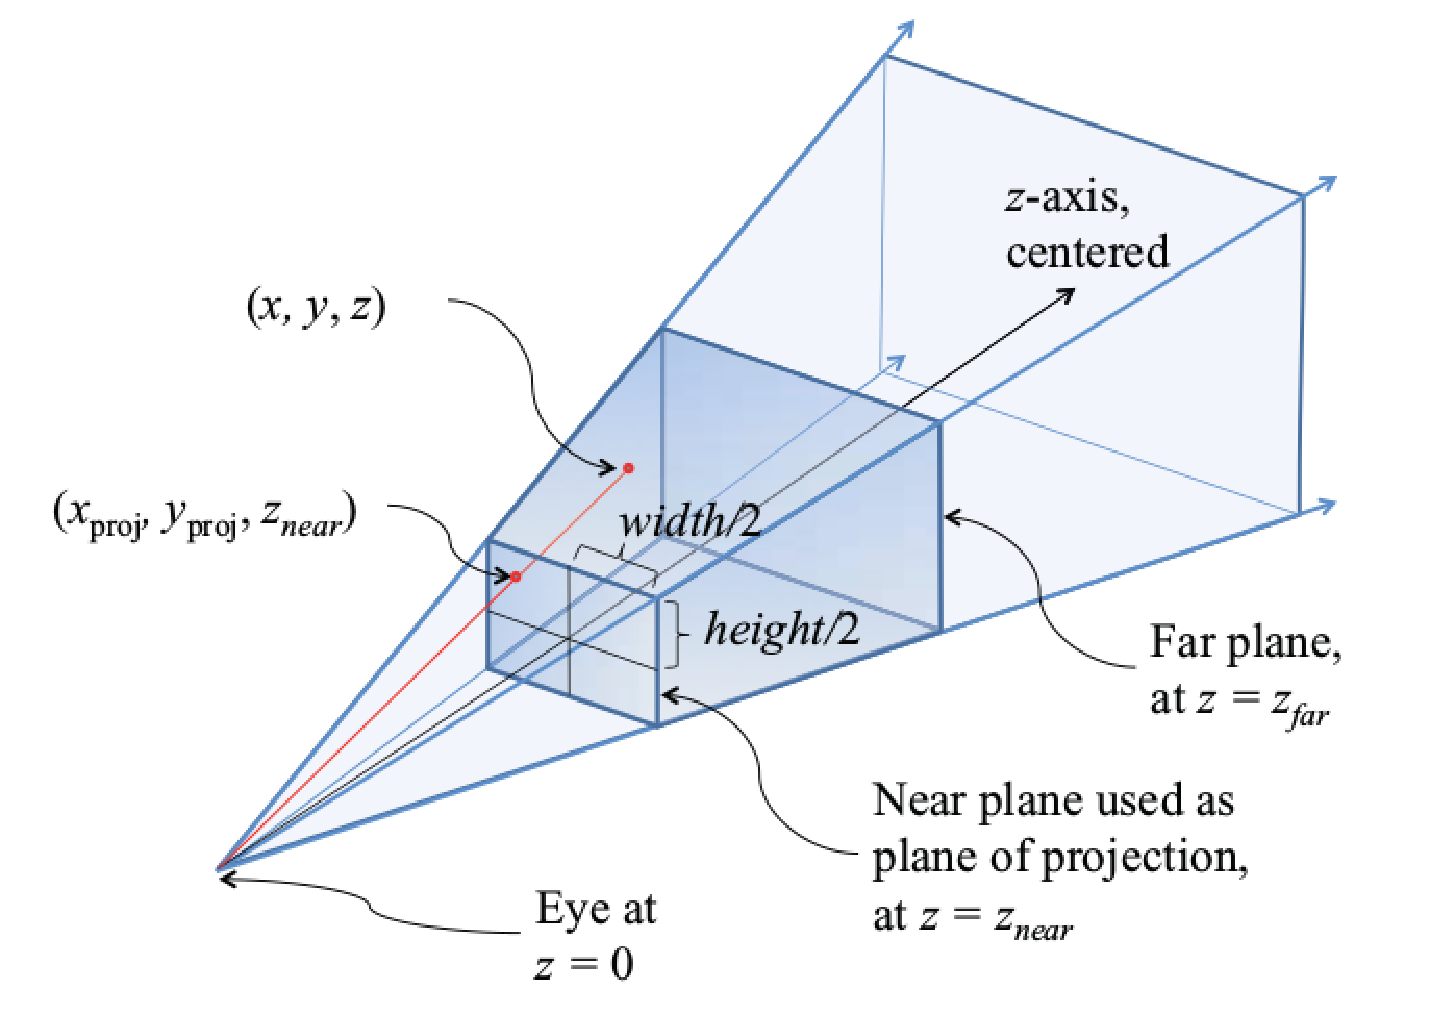
\includegraphics[width=0.6\textwidth]{perspective_projection}
    \caption{Perspective projection with combined projection plane and near clipping plane}
    \label{fig:perspective_projection}
\end{figure}

\subsection{Perspective projection}

As seen in Figure~\ref{fig:perspective_projection}, perspective projection has a lot in common with the pinhole projection. This makes the projection carry a sense of depth in the image. Objects closer to the near clipping plane becomes larger, and objects further away becomes smaller. The focus point at the origin represents the human eye, and how it would perceive the projected world.

To make the projection map to each pixel on a screen \todo[inline]{insert maths. need reference matrices}

%%% Need to replace the rest %%%
\subsection*{\#\#\#to be fitted into perspective projection\#\#\#}
Normal graphics projection from scaled from meters to $x,y,x \in [-1,1]$:

\begin{equation}
    Proj\_mat = \begin{bmatrix}
        \frac{AR}{tan(\frac{\theta}{2})}    &   0                                   &   0   &   0   \\
        0                                   &   \frac{1}{tan(\frac{\theta}{2})}    &   0   &   0   \\
        0                                   &   0                                   &   -\frac{n+f}{n-f} & 1\\
        0                                   &   0                                   &   \frac{2nf}{n-f} & 0
    \end{bmatrix}
\end{equation}

where $AR$ is the aspect ratio $\frac{Width}{Height}$, $n$ is the near clipping plane and $f$ is the far clipping plane. $\theta$ is the field of view. Here Horizontal field of view is equal to the vertical field of view.


\subsection{Othographic projection}

Orthographic projection differ from perspective projection in the sense that all projection lines are parallel. As we see in Figure~\ref{fig:orthographic_projection}, this means that there is no focus point for the projection lines, but rather just a view direction. This causes the relative sizes in the image to be preserved, making the projection type ideal for schematics and applications that require measurements.

\begin{figure}[!htb]
    \centering
    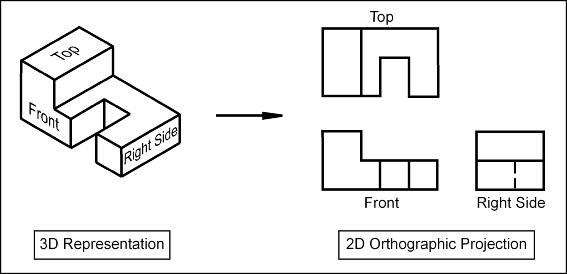
\includegraphics[width=0.5\textwidth]{3d_ortho}
    \caption{Orthographic projection}
    \label{fig:orthographic_projection}
\end{figure}



%%%% NEED TO BE REWRITTEN AND PLACED SOMEWHERE

\section{TEMP\_PLACEMENT...Structuring 360 degree data}
360 degree picture data representations are highly based on the type of camera used to cature it: A fisheye lense will make a circle in the rectangular matrix representation, causeing a lot of black "dead" spots with no information. The same type of representation is gained from using a Catadioptric lens. However this also removes the middle of the picture, because of the way it is constructed.

Another way to represent a picture is by a unit-sphere coordiante system. Using a $\phi$~-~$\theta$ map, instead of pixels. This $\phi$~-~$\theta$ representation usually maps to a pixel on a cube or stitched image, assuming the different cameras have a common focal point. You can also go directly from a pinhole, fisheye, catadioptric or some other representation to a sphere representation. This will just cause non-captured parts to be black.

Low level structure comes down to a list, matrix, struct or class of some sort, maybe with compressing. Accessing and iterating over these structures however can be done in different ways: 

\subsection{Fisheye and Catadioptric representation}
This method of structuring uses the maps the catured image directly to a rectangular data structure; eg. matrix. The representation is directly coupled to pixels, rather than angles and distances. To get this information, we have to recreate it from a camera model.

\textbf{Pros:}
\begin{itemize}
    \item Easy to implement
    \item Easy to iterate over
\end{itemize}

\textbf{Cons:}
\begin{itemize}
    \item Harder to visualize for humans. 
    \item Need extra functions to get real world positions
    \item Pixels gets mashed or streched, potentially removing information from the picture.
\end{itemize}

\subsection{Unit sphere representation}
The low level implementation of this method is still a matrix-like data structure. However, the indexes of the matrix is now the spherical angles $\phi$ and $\theta$. This causes each matrix value to represent a color value in a specific direction from the center point.

\textbf{Pros:}
\begin{itemize}
    \item Easier for humans to visualize if a 3D-sphere picture is produced.
    \item Easy to iterate over
    \item Depending on the cameras used to make this representation, you may preserve more picture details.
    \item Easiest implementation for image stitching
    \item Real world coordinates directly represented in data array indices. 
\end{itemize}

\textbf{Cons:}
\begin{itemize}
    \item Need extra post-processing of image data. 
    \item Distortions will be stretched out and amplified, if you convert from fisheye or catadioptric.
\end{itemize}

\subsection{Etended Unit sphere representation}
By defining a class containing a storage data structure, and functions for accessing it. Main goal of the representation is to "remove" edges of the picture, since the edge wraps around to the other side like a sphere.


%===================================== CHAP 3 =================================

\chapter{Simulator for 360 degree fisheye lens image capture on an UAV} \label{chap:simulator}

This chapter shows the implementation of a camera simulator for capturing omnidirectional fisheye lens images in Unreal Engine, building upon an already existing robotics simulator plugin called AirSim\footnote{github.com/Microsoft/AirSim} \cite{Airsim_paper}. The existing simulator is augmented with a ROS\footnote{ros.org/} interface, an omnidirectional camera model, with modelled fisheye lens distortion and the ability to transform and combine the perspective pictures captured, into a singe wide angle fisheye lens distorted image. For now the simulator will only supporrt the equidistant distortion model, and will be made to mimic real calibrated camera models, for example through the Kalibr\footnote{github.com/ethz-asl/kalibr/} toolbox.

The chapter is split into two parts: The first sections will show related work on camera simulators for robotics and current advancements in the field, as well as discuss relevant platforms to base the omnidirectional camera simulator on. The second part will go deeper into the implementation of the simulator itself, with a focus on the augmentations done within the scope of this project.

\section{Related work} \label{sec:simulator_related}

As mentioned in Section~\ref{chap:introduction}, there ha been a lot of recent development within the area of computer vision for use with UAVs, which has also produced the need for realistic simulators to ease the testing process, decrease costs and increase the efficiency. Some simulators are built from ground up, like V-REP \cite{VREP2013} and Gazebo \cite{GazeboPaper}. While these are general purpose robotics simulators, there are multiple projects extending these simulators to connect to other interfaces or concentrate on spesific tasks. For example RotorS\footnote{github.com/ethz-asl/rotors\_simulator} \cite{RotorS}, which is a simulator for control and state estimation of MAV or Micro Aerial Vehicles. This simulator is built on top of Gazebo and Gazebo's ROS interface, adding MAV and Sensor models, while extending Gazebos capabilities for MAV control and state estimation.

Since 2010 there has also been an increase in the use of game engines and other graphically capable software to help increase the realism of computer vision simulators. HNMSim \cite{HNMSimPaper} is made for simulating networks fo UAVs, and combined the use of Matlab, Simulink and LabView with the game engine Unreal Engine and 3D modeling software Autodesk 3Ds Max, to create more realistic environments for the simulations. They also implemented and simulated a multirotor with an attached camera in Unreal Engine. Another simulator\cite{UnityROSsim}, created by Meng et al, built upon the Unity game engine. They implemented a multirotor and a LIDAR model, with a ROS interface to communicate to externally and use control algorithms made for ROS.

In 2017, two simulators for simulating autonomous vehicles in realistic environments were released. Sim4CV \cite{Sim4CV_paper} and AirSim \cite{Airsim_paper}. Both of these implement a multirotor and a car model, using Unreal Engine as a their original backend. It should be mentioned that in late 2018, Microsoft started developing AirSim for Unity as well, and it looks like they will support both engines going forward. Both of these will be discussed in more detail in Section~\ref{sec: UnityUnreal} and \ref{sec:Chooseplatform}.

While experiments have been done using real or synthetic picture datasets, taken with fisheye or catadioptric cameras, have shown that it can be beneficial to use over normal perspective cameras \cite{Zhang2016BenefitOL, OmniVIOKalman, CompOmniVSLAM}, there are no realeased open source simulators for 360 degree camera captures with the possibility for closed loop operation. One probable reason for this is that only perspective camera models have been implemented in most simulators. There was a promising looking project implementing a 360 degree fisheye camera for Gazebo shown as a tutorial at Gazebo's tutorials page \cite{GazeboWideWeb}. However this seems to have been removed recently, as it is no longer available. Both Unity and Unreal Engine on the other hand support capturing scenes to cubemaps. Cubemaps are made of 6 images with a common focus point for their projction, covering all directions in the scene. This has been used to capture 360 degree video, as seen in \cite{UnityCubeCapture, UnrealCubeCapture}, although it has not been implemented as a part of either of the simulators mentioned. 

The simulator in this project will be based on a previously developed simulator, and will focus on implementing 360 degree camera capture to work with the already existing framework. Due to a lack of experience with simulators and game engines, there will only be a focus on open software, with a sizeable community, and that are still used and supported by the developers. All of Gazebo, Unreal Engine and Unity match this criteria. For this reason, these platforms will be compared as alternatives. An important note is that this comparison should not be treated as comprehensive comparison of the different simulators or game engines mentioned, and far from all features will be mentioned in this chapter. This comparison is just a result of the initial research done, in order to make a omnidirectional camera simulator for robotics applications.

\section{Gazebo} \label{sec:Gazebo}

Gazebo is a simulator platform made for robot simulation, with 3D graphics for Linux platforms, and can be built with four different physics engines \cite{Gazebo_phys}. The four engines are optimized for different purposes, making Gazebo quite versatile when it comes to simulations. Gazebo is fully usable as a standalone, but it also comes with native ROS support. This means that you can model your hardware in Gazebo and run the same ROS code with this model, as you would with the physical robot.

The simulations in Gazebo are built from XML-files describing the world, models that inhabit the world, and the physical properties of each model. The models can be attached to one another through joints and links to create more complex models. Gazebo also provides the ability to add specific behaviour to the simulation through plugins. Plugins are compiled C++ code attached to a specific component, like a model, sensor or world. It is also through these plugins you define ROS behaviour.

The camera sensor implements a perspective camera, giving you access to the typical camera parameters: horizontal FOV, image height, image width, color coding, and near and far clipping plane. Gazebo also comes with support for adding Gaussian noise and distortion to the camera. The distortion is based on Brown's distortion model\cite{BrownModel}, which models both radial and tangential distortion effects to the output picture. There are no shutter speed settings, meaning that motion blur and exposure time settings are not naturally supported.

\begin{figure}[!htb]
    \centering
    \begin{subfigure}{0.45\textwidth}
        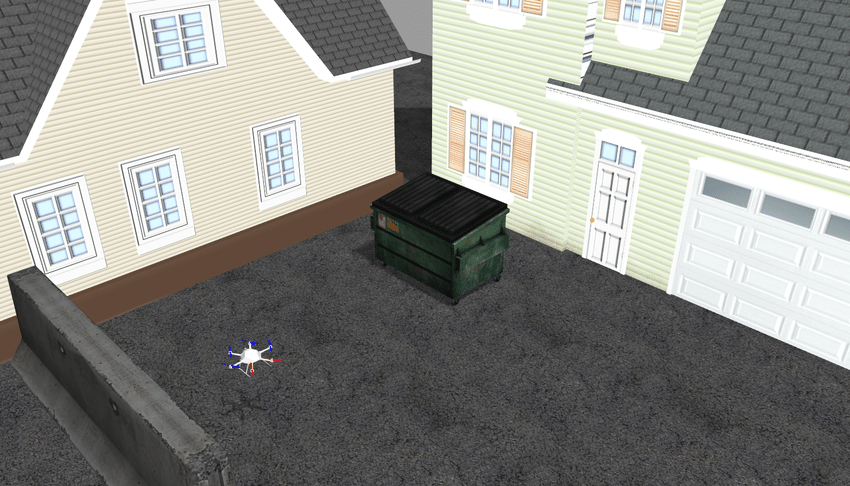
\includegraphics[height=4cm]{rapport/fig/Simulator/A-screenshot-of-the-RotorS-simulator-The-scene-is-built-up-from-Gazebo-default-models.png}
        \caption{From RotorS simulator paper \cite{RotorS}}
        \label{fig:A}
    \end{subfigure}
    \begin{subfigure}{0.45\textwidth}
        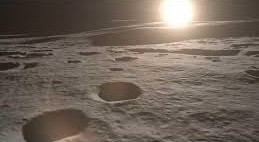
\includegraphics[height=4cm]{rapport/fig/Simulator/gazebomoon.jpg}
        \caption{Moon simulation by NASA \cite{NASAGazeboppt}}
        \label{fig:NASA_Gazebo_moon}
    \end{subfigure}
    \caption{Comparison Gazebo simulations with built-in shader(left) and custom shader(right). The simulation on the right also implements custom imported materials.}
    \label{fig:Gazebo_imgs}
\end{figure}

Another drawback of Gazebo is its graphical capabilities of the built-in model editor. Although you may import meshes and textures from other 3D modeling software, there are limited ways of editing these inside the editor. This makes it difficult to create realistic scenes. This is especially true when it comes to implementing vegitation and foliage, like grass, trees and flowers, as these require fine tuning together with the other elements in the scene to look good. The capability of the shader is also quite limiting compared to other 3D modeling software, meaning that it is hard to create realistic light settings. Especially with multiple light sources. There is however support for using custom shaders, as NASA did in this example \cite{NASAGazeboppt}, showing that it is posible to augment the capabilities of Gazebo to produce good results. Figure~\ref{fig:Gazebo_imgs} shows a comparison between two environments made in Gazebo. The left picture shows an environment from the RotorS simulator, using mostly built-in models and materials, while the right picture shows a custom imported environment with a custom built shader.

\section{Unity and Unreal Engine 4} \label{sec: UnityUnreal}

Unity and Unreal engine are the most popular game engines freely available. Being game engines, both heavily focus on productivity in graphics design, as well as visuals of the final product. This means that a large part of the software toolkit is based around editing the scene and objects in it to look good. Both engines provide extensive tools for making custom meshes, textures, animations and lighting effects, making the graphical development of the simulation much easier than in Gazebo. In addition to this both Unity and Unreal Engine provide a large library of premade scenes to use freely, in addition to a marketplace where you can buy assets others have made. Figure~\ref{fig:showcase_unityunreal} shows two images of scenes made in Unity and Unreal Engine. Rendering scenes of this quality will of course require more powerful hardware than what is needed for Gazebo, especially for real time simulations, but the pictures shows the power of the tools provided in these engines. 

\begin{figure}[!htb]
    \centering
    \begin{subfigure}{0.45\textwidth}
        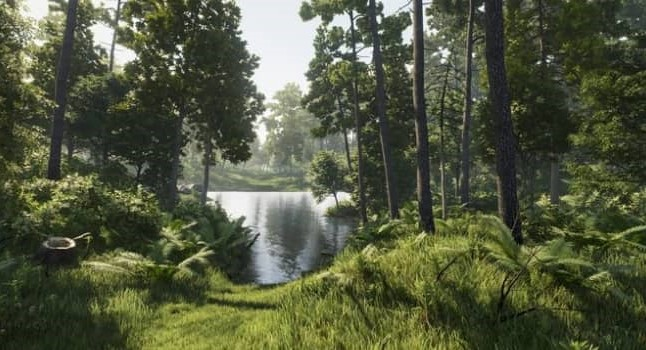
\includegraphics[height=3.8cm]{rapport/fig/Simulator/unrealforest.jpg}
        \caption{Made by Michal Franczak using the UE4 editor \cite{Unrealshowcase}}
        \label{fig:unreal_forest}
    \end{subfigure}
    \begin{subfigure}{0.45\textwidth}
        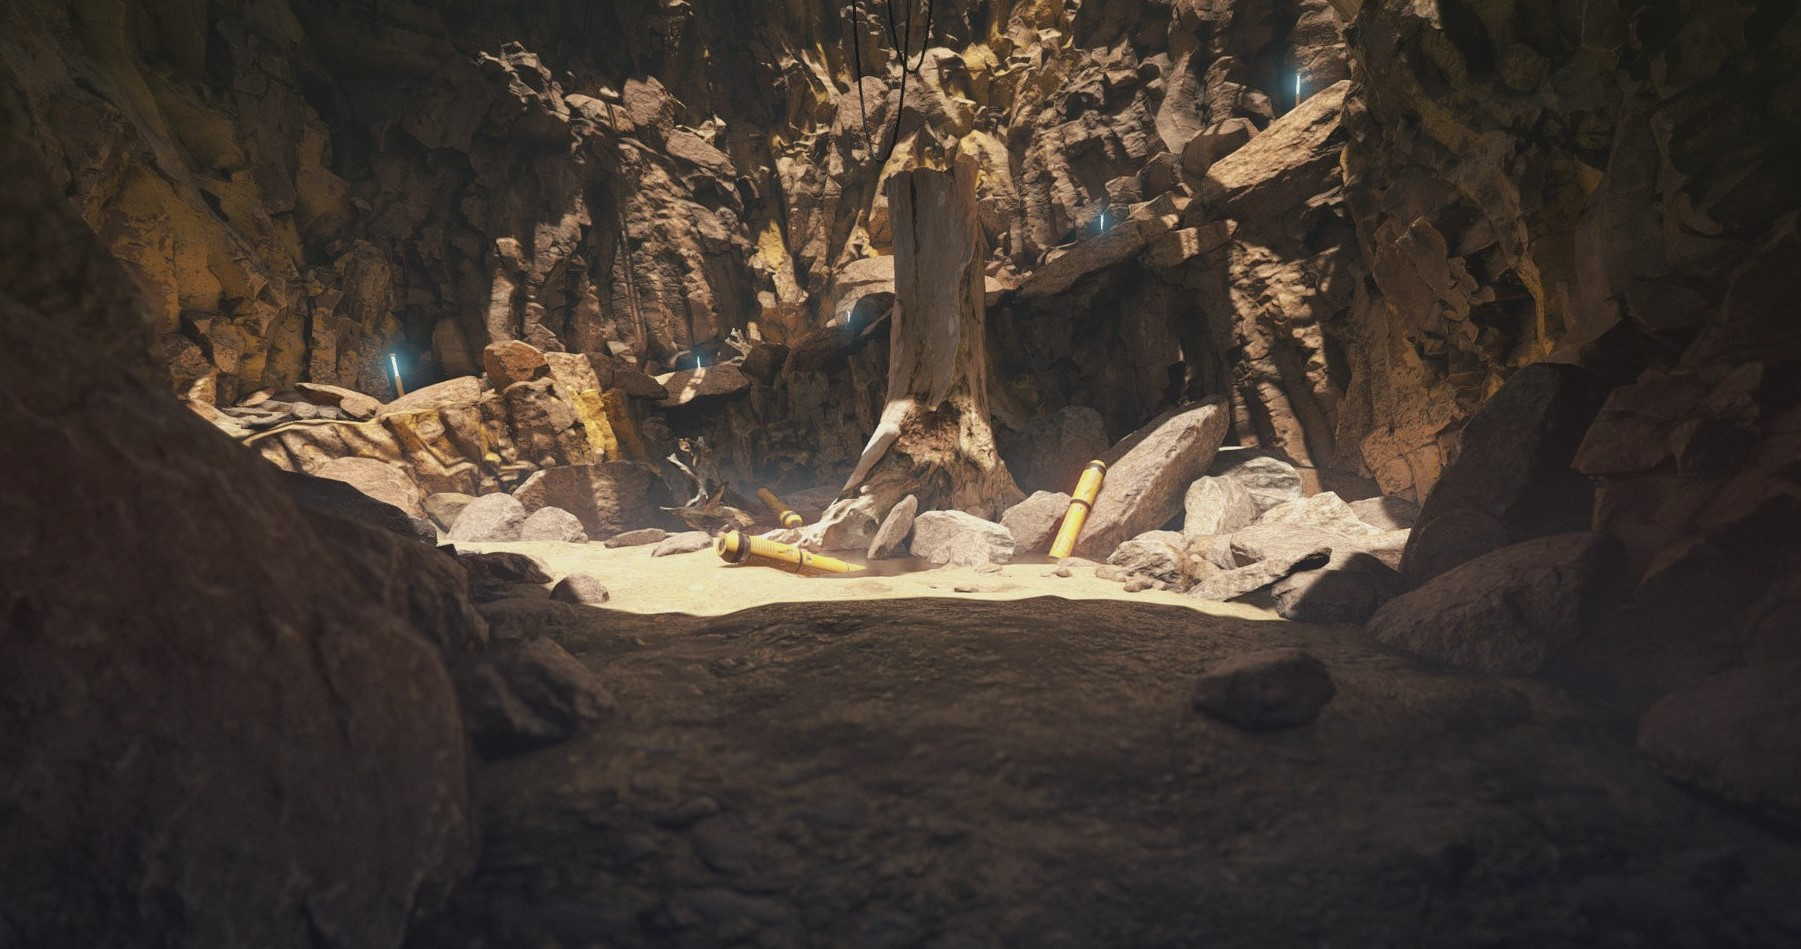
\includegraphics[height=3.8cm]{rapport/fig/Simulator/unitycave.jpg}
        \caption{Created by Pat Goodwin using the Unity editor \cite{Unityshowcase}}
        \label{fig:Unity_cave}
    \end{subfigure}
    \caption{Showcase of two quite realistic looking environments created in Unreal Engine 4 (left) and Unity (right)}
    \label{fig:showcase_unityunreal}
\end{figure}

Unity is based around the scripting language C\# to change the behaviour of the object. The script itself is then attached to a spesific object. The behaviour is defined through five user defined functions: $Awake()$, $Start()$, $Update()$, $FixedUpdate()$, and $LateUpdate()$. The $Awake()$ and $Start()$ functions are called once, while the rest are called every frame. Most importantly we note that $FixedUpdate()$ is specifically used for updating physics, while $Update()$ is for general purpose updates. However, it is not required to use the provided physics engine.

Unreal Engine is built quite similarly to Unity in regards to the building blocks of the Editor. However, there are two ways to define behaviour. One is through C++ and the other is through a visual scripting language called Blueprints. The functionality of Blueprints are almost identical to that of the C\# scripting in Unity, however the programming interface is graphical and node based, as seen in Figure~\ref{fig:blueprint_editor}. The complete source code of Unreal Engine freely available, and you are allowed to make changes to the engine itself. Through registering as a Epic Games developer, you get access to all features of Unreal Engine through the C++ source code. This enables the ability to apply extra optimizations for your specific problem, and may be relevant for performance critical tasks. The same interface available to the blueprints are also available to C++, giving you the ability to do scripting similar to that of Unity.

\begin{figure}[!htb]
    \centering
    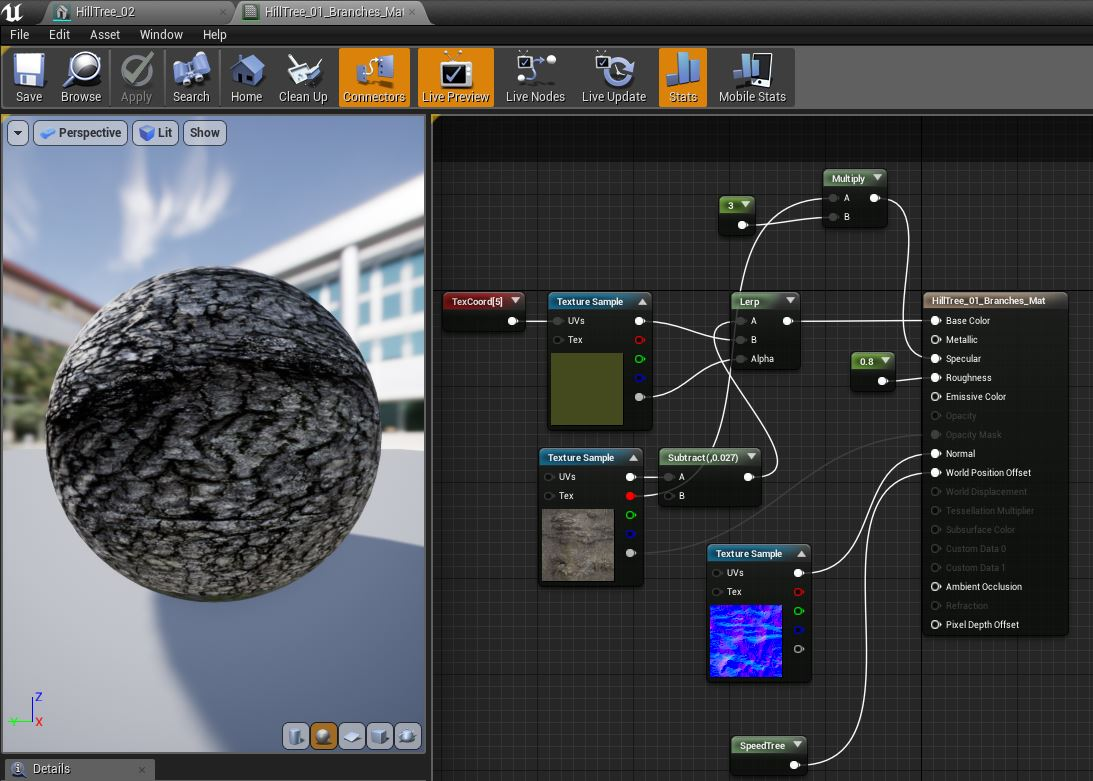
\includegraphics[height = 6cm]{rapport/fig/Simulator/blueprintprog.JPG}
    \caption{Partial picture of UE4 Blueprint for tree branch texture}
    \label{fig:blueprint_editor}
\end{figure}

Both Unreal Engine and Unity comes with a physics engine, and usage of this engine is completely optional. This is very different from the implementation in Gazebo, where physical properties like mass, inertia are core parts of a model. While the engines do implement solvers for collision, interaction through joint and links and physical properties, there are no initial support for simulation of wind or other fluid mechanics.

When it comes to computer vision applications, there are no native support for this in the engines. This may be solved by using OpenCV\footnote{https://opencv.org/} as a part of the project. There exists a wrapper for OpenCV in Unity, and you may link the OpenCV libraries directly into your Unreal Engine projects through C++ code. OpenCV provides many computer vision algorithms as well as algorithms for machine learning, and can be used to augment the engine's cameras for wide angle functionality, lens distortions or similar effects. To get an interface to create image datasets from Unreal Engine, a plugin has been created called UnrealCV~\cite{UnrealCV}. This plugin does not support omnidirectional captures or lens models at the moment.

Sim4CV and Airsim both simulators implement model for an quadcopter and a car. While Sim4CV is written directly into Unreal Engine, AirSim is available as a plugin for both Unreal Engine and for Unity. According to the paper realeased with Sim4V, this fact limits the capabilities of the physics simulations of AirSim \cite{Sim4CV_paper}, though I have no additional data to back that up. Since AirSim is a plugin, it is possible to integrate with existing projects, and the procedure is well documented in their Github repository. This means that it is relatively easy to integrate AirSim into environments created by others, without AirSim in mind. 

When it comes to interfacing, both simulators implement an API for Python, as well as C++. Sim4CV also implements an API for MATLAB\footnote{www.mathworks.com/products/matlab.html}, which might be useful since MATLAB has lots of CV toolboxes available through the NTNU licence. Though none of them directly implements an interface to ROS, there are examples of simple ROS communication with AirSim in their repository.

Though both simulators implement much of the same features, the differences between the two come in the form of their main focus. Sim4CV focus on computer vision, and the usage of computer vision for machine learning and deep learning, while AirSim mainly focuses on supporting different types of sensors. This means that for projects aiming for sensor fusion, or testing complete vehicle systems, AirSim would be preferred. Sim4CV may on the other hand be preferrable for AI computer vision projects. Especially for deep learning, as it implements a TensorFlow-like interface.

\section{Choosing a platform for the simulator} \label{sec:Chooseplatform}

As mentioned at the start of this chapter, the goal of this project is to implement a simulator for capturing realistic 360 degree images with fisheye lenses, with the ability to calibrate the camera parameters to match real fisheye lens cameras and solutions to capture 360 degree footage. In addition, the simulator should provide an interface to ROS~\cite{ROSpaper}, to enable the simulator to be used with already existing implementations of SLAM and Visual odometry algorithms for ROS. This criteria limits the usage to Linux based systems, as ROS are currently only available on Linux platforms. While Unity and Unreal Engine are most optimized for development on Windows or Mac OS, both provide the ability to build their latest releases on Linux. Table~\ref{tab:comparison_interface} shows a comparison of the interfaces of Gazebo, Unity and Unreal Engine.

\begin{table}[!htb]
    \centering
    \begin{tabular}{|c|>{\centering\arraybackslash}m{2cm}|>{\centering\arraybackslash}m{2cm}|>{\centering\arraybackslash}m{2.8cm}|>{\centering\arraybackslash}m{2cm}|>{\centering\arraybackslash}m{2cm}|>{\centering\arraybackslash}m{2cm}|>{\centering\arraybackslash}m{2cm}|} \hline
        \textbf{Software}          & \textbf{OS}  & \textbf{ROS} & \textbf{Model/Scene toolbox}   & \textbf{Sensor models} & \textbf{Language}              \\ \hline \hline
        Gazebo          & Linux           & Yes           & Simple  & Yes & C++, XML                 \\ \hline
        Unity           & Windows, Mac OS, Linux                    & No            & Extensive & Plugins & C\# \\ \hline
        Unreal Engine   & Windows, Mac OS, Linux  & No            & Extensive & Plugins/ custom versions & C++, Blueprint \\ \hline
    \end{tabular}
    \caption{Interface comparison of Gazebo, Unity and Unreal Engine}
    \label{tab:comparison_interface}
\end{table}

The main advantages Gazebo has over the game engines is its implementation of multiple physics engines, its ROS integration and its modular sensor setup. A larger part of the community is also familiar, and uses Gazebo for computer vision purposes, which may provide more useful help online for the project. The main drawback of Gazebo is that there is limited tooling for graphical development. This means that there are relatively few high quality scenes made for Gazebo. Making these from scratch would require much more time and experience, as well as additional graphical software, which is unreasonable for the scope of this project. 

The tools available in the Unreal Engine and Unity, provide a much easier way to make high quality scenes for our camera, or editing scenes that are readily available. The fact that both of these engines also support omnidirectional video capture through cube maps, may also be helpful when implementing the 360 degree camera feature. In Table~\ref{tab:comparison_camera} we see that Gazebo has the most advanced distortion model. This is true even with the extra functionality provided by AirSim and Sim4CV. Additional post processing of the images must therefore be applied to the images, to obtain the same distortion effects. The main advantages of Unity and Unreal Engine is their advanced shader and post processing unit, which can capture multiple effects seen in normal cameras, like motion blur caused by the combination of a large exposure time and movement.

\begin{table}[!htb]
    \centering
    \begin{tabular}{|c|>{\centering\arraybackslash}m{4cm}|>{\centering\arraybackslash}m{4cm}|>{\centering\arraybackslash}m{4cm}|} \hline
        \textbf{Camera} & \textbf{Gazebo} & \textbf{Unity} & \textbf{Unreal Engine} \\ \hline\hline
        Camera type     & Perspective & Perspective, Cubemaps & Perspective, Cubemaps \\ \hline
        Distortion model & Radial, Tangetial & Radial  & "Panini Distortion"\cite{panini} \\ \hline
        Noise           & Yes & Yes & Yes \\ \hline
        Exposure time   & No & Yes & Yes \\ \hline
        Motion Blur     & No & Yes & Yes \\ \hline
        Vignette        & No & Yes & Yes \\ \hline
        
    \end{tabular}
    \caption{Camera comparison of Gazebo, Unity and Unreal Engine}
    \label{tab:comparison_camera}
\end{table}

The shader of Unreal Engine and Unity is also significantly better at lighting, creating shadows and handling reflections. In Gazebo only directional light sources cast shadows. These are light sources like the sun, where all light rays are close to parallel. In the game engines however, all sources of light do. This means that the the shadows cast in the scene will act more natural, and you will also naturally get effects like multiple shadows of differing intensity appear when being near multiple sources of light. The supported area lighting also casts softer shadows, as they would in the real world. Creating similar effects in Gazebo would only be possible by writing a custom shader. Table~\ref{tab:comparison_shader} shows a comparison of the built- in shaders. The additional sky light tool in Unreal Engine is a special form of directional light, meant to simulate the effect of sunlight outdoors.

\begin{table}[!htb]
    \centering
    \begin{tabular}{|>{\centering\arraybackslash}m{3cm}|>{\centering\arraybackslash}m{3.5cm}|>{\centering\arraybackslash}m{4cm}|>{\centering\arraybackslash}m{3.5cm}|} \hline
        \textbf{Shader effects} & \textbf{Gazebo} & \textbf{Unity} & \textbf{Unreal Engine} \\ \hline\hline
        Light types     & Lightmaps, Directional, Spot, Point, Ambient & Lightmaps, Directional, Spot, Point, Area, Ambient, Fluorescent & Same as Unity + Sky Light \\ \hline
        Shadow Generation & Directional light sources & All light sources & All light sources \\ \hline
        Ambience        & Yes & Yes & Yes \\ \hline
        Chromatic abberation & No & Yes & Yes \\ \hline
        Ambient occusion & No & Yes & Yes \\ \hline
        Light shafts    & No & Yes & Yes \\ \hline
        Bloom/lens flare & No & Yes & Yes \\ \hline
        Reflection      & No & Yes & Yes \\ \hline
    \end{tabular}
    \caption{Built-in shader capabilities of Gazebo, Unity and Unreal Engine}
    \label{tab:comparison_shader}
\end{table}

As the scope of this project mostly includes image capture, and the fact that there are multiple effects that appear in real world photography that cannot be reasonably recreated in Gazebo, the main platform of this project will be a game engine. To write my own shader for Gazebo is also too much work for one person to do withing a few months, without any previous experience in the field. Since omnidirectional image capture is not implemented in any of the platforms, that has to be done no matter which platform is chosen. Writing a lens model for adding distortions to companion that, should be managable.

Unreal Engine has some advantages over Unity. The fact that you may write C++ code directly, increases the ability to use libraries like OpenCV without needing additional wrappers. It also simplifies the process of making a ROS interface, as the ROS projects are also compiled from C++ code. Although AirSim started supporting Unity in late autumn 2018, it was only available for Unreal Engine 4 at the start of this project. As I did not find any equivalent plugins for Unity, Unreal Engine was chosen as the simulator platform. AirSim was also chosen over Sim4CV because of the availability of the source code on Github, making it easy to see that the project was still developed and had a sizeable user base. The versatility it provides for additional sensors is also something that may be utilized in future projects.


\section{System overview}

This project will be set up as three main modules: Unreal Engine, AirSim and the fisheye camera. These are all compilable as their own packages, and does not need to be compiled in any specific order. Only Unreal Engine is executable on its own. AirSim is indirectly run by AirSim through adding the plugin to a specific unreal project, while the AirSim enabled project needs to be running within Unreal Engine in order to run or use the fisheye module. 

The AirSim plugin is made in a way so that it technically resides outside of Unreal Engine. However, it has full access to the resources of the Engine, through the engine's header files. Their design choice involves adding as much functionallity as possible outside of the Engine, to make it easier to support other game engines with only small changes to the AirSim package. The added features in the AirSim package includes: Multirotor and car models, perspective and depth camera, LIDAR, IMU with magnetometer and GPS. In addition to this it supports hardware in the loop(HITL) through the PX4/Pixhawk flight controller and MAVlink. 

As of now, AirSim is only usable with version 4.18 of Unreal Engine, while 4.21 is available at the time of writing. In order to reduce the chances of new commits to the original repositories causing problems for my project. Both AirSim and Unreal Engine 4.18 have been forked to a separate repository. This allows for full control over the updates made to the original repositories in addition to allowing custom modifications. The modifications to AirSim are available publicly. However, any changes to Unreal Engine must be kept private due to licencing.

\subsection{Communication pattern}

Because of the design choices of AirSim, much of the simulator computations happen outside of Unreal Engine. While Unreal Engine handles the core game loop, resource management and the graphical tasks, custom AirSim scripts handle sensor simulation and kinematics. Of course, AirSim also relies on Unreal Engine for camera data, actor positions and pose, in addition to timing data. The AirSim plugin implements a game mode which is run by Unreal Engine on simulation start. This decides whether to do a multirotor simulation, car simulation or computer vision mode. The computer vision mode turns off physics, enabling free camera movement for creating datasets. The game mode also sets up the program loop run for each actor each frame.

The API AirSim consists of a server/client based system, using the remote procedure call(RPC\footnote{https://github.com/rpclib/rpclib}) library. This enables messages to be sent as network packages(TCP/IP), in addition to allowing interfaces made for multiple programming languages. The server is written in C++, and the client side is implemented for both Python and C++. As long as the server is enabled in the configuration file, it is started by Unreal Engine on simulation startup. 

\begin{figure}[!htb]
    \centering
    \begin{tikzpicture}[node distance=2.2cm, transform shape, scale=0.7]
        \tikzstyle{topblob} = [ellipse, minimum width = 7cm, minimum height = 2cm, text centered, draw=black, fill=blue!10]
        \tikzstyle{blob} = [ellipse, minimum width = 3cm, minimum height = 1.5cm, text centered, draw=black, fill=red!20]
        \tikzstyle{emphblob} = [ellipse, minimum width = 3cm, minimum height = 1.5cm, text centered, draw=black, fill=red!50]
        \tikzstyle{ownblob} = [ellipse, minimum width = 3cm, minimum height = 1.5cm, text centered, draw=black, fill=green!10]
        \tikzstyle{doublearrow} = [thick, <->, >=stealth]
        \tikzstyle{tcp} = [dashed]
        
        \node (UE) [topblob]{Unreal Engine};
        \node (AirSim) [blob, below of=UE, align=center, yshift=-0.5cm]{AirSim \\ Plugin Core};
        \node (Sens) [blob, left of=AirSim, align=center, xshift=-3cm]{Sensor \\ Models};
        \node (Phys) [blob, below right of=AirSim, align=center, xshift=3cm]{Physics \\ Engine};
        \node (cam) [emphblob, above of=Phys, align=center, yshift=0.5cm]{\textbf{Camera} \\ \textbf{Interface}};
        \node (RPCS) [blob, below of=AirSim]{RPC Server};
        \node (RPCC) [blob, below of=RPCS]{RPC Client};
        \node (Client) [ownblob, below of=RPCC]{Core loop};
        \node (Fish) [ownblob, right of=RPCC, xshift=3cm, align=center]{Fisheye \\ Transform};
        \node (ROS) [ownblob, left of=RPCC, xshift=-3cm, align=center]{ROS Publisher};
        
        \draw[doublearrow] (UE) -- (AirSim);
        \draw[doublearrow] (UE) -- (Sens);
        \draw[doublearrow] (UE) -- (cam);
        \draw[doublearrow] (AirSim) -- (Phys);
        \draw[doublearrow] (AirSim) -- (cam);
        \draw[doublearrow] (AirSim) -- (Sens);
        \draw[doublearrow] (AirSim) -- (RPCS);
        \draw[tcp] (RPCS) -- (RPCC); \node (tcpText) [left of=RPCC, , xshift=1cm, yshift=1.1cm]{\scriptsize TCP/IP};
        \draw[doublearrow] (RPCC) -- (Client);
        \draw[doublearrow] (Client) -- (Fish);
        \draw[doublearrow] (Client) -- (ROS);
        
    \end{tikzpicture}
    \caption{Simplified code interaction within the simulator. Red nodes belong to the AirSim plugin, while Green nodes are custom made for this project. The emphasized node represent modified AirSim code.}
    \label{fig:comm_pattern}
\end{figure}

The project will be implemented for the multirotor game mode. This means that it will not run on the other game modes. The reason for this is that the cameras need to be set up specifically for each game mode, through the Unreal Engine Blueprints imported by the game mode. The fisheye camera and ROS interface will depend on the C++ RPC client API, the perspective camera model and the image capture module for AirSim. The contribution of the project will be to combine perspective images into a single fisheye lens distorted image, with as few changes as possible to the AirSim plugin. In addition to this it will build upon the C++ API to allow for publishing images to ROS, through the normal ROS publisher interface. Figure~\ref{fig:comm_pattern} shows the main communication flow of Unreal Engine, AirSim and the fisheye camera. As the project does not involve HITL with PX4, Mavlink or any controller setup, they are not shown in the figure, and will not be discussed any further in this report.

\section{Implementation}

The goal of the implementation is to get a fisheye camera working, and to to publish the images to ROS. As only perspective cameras are available, and that they are mounted to specific parts of the multirotor, it was not possible to implement this without making changes to AirSim. However, it was decided early on that no changes would be made to the source code of Unreal Engine. While some changes had to be made to the API in order to implement the ROS node, all of the old API is still functioning and usable.

\subsection{Early development} \label{sec:Early_dev}

As described in Section~\ref{sec:simulator_related}, Unreal Engine support capturing of cubemaps, which is a technique of capturing the whole scene through rendering six $90^\circ$ FoV pictures. These are then strored in a special structure, with tooling for projecting it onto a sphere or plane trough equireclinear projection. As the texture mapping tool for cubemaps incorporate radial distortion, it was a natural starting point for simulating fisheye lenses. It is also used in \cite{UnrealCubeCapture}, where they describe using it in their omnidirectional video for their game.

There are various tutorials of how to capture $360^\circ$ screenshots, and many of them are using the Nvidia Ansel plugin \cite{SceenshotsAnsel}. While this made equireclinear captures of the scene, there was no way of processing the images directly, outside of saving them locally and loading the images through OpenCV or by similar means. While this is definitely possible, it would create unecessary save and load cycles. In addition to this, the performance of saving and loading images from disk varies heavilly from computer to computer.

\begin{figure}[!htb]
    \centering
    \begin{tikzpicture}[node distance=3.5cm, transform shape, scale=0.7]
        \tikzstyle{topblob} = [ellipse, minimum width = 7cm, minimum height = 2cm, text centered, draw=black]
        \tikzstyle{blob} = [ellipse, minimum width = 3cm, minimum height = 1.5cm, text centered, draw=black]
        \tikzstyle{singlearrow} = [thick, ->, >=stealth]
        
        \node (cap) [topblob]{SceneCaptureComponent};
        \node (cap2d) [blob, below left of=cap, align=center]{SceneCapture- \\ Component2D};
        \node (cap3d) [blob, below right of=cap, align=center]{SceneCapture- \\ ComponentCube};
        \draw[singlearrow] (cap) -- (cap2d);
        \draw[singlearrow] (cap) -- (cap3d);
        
        \node (rend) [topblob, right of=cap, xshift=8cm]{TextureRenderTarget};
        \node (rend2d) [blob, below left of=rend, align=center]{TextureRender- \\ Target2D};
        \node (rend3d) [blob, below right of=rend, align=center]{TextureRender- \\ TargetCube};
        \draw[singlearrow] (rend) -- (rend2d);
        \draw[singlearrow] (rend) -- (rend3d);
        
    \end{tikzpicture}
    \caption{Unreal Engine Capture Component and Render Target class inheritance.}
    \label{fig:capture_render_inherit}
\end{figure}

The second approach involved modifying the capture request and processing system in AirSim directly, to allow requests of both perspective images and cubemaps through the existing API. Each camera actor in Unreal Engine needs a capture component and a render target in order to know what to capture and where to store the data. In AirSim's camera setup and API, only the 2D version shown in Figure~\ref{fig:capture_render_inherit} is implemented. Adding support for cube captures would therefore either mean to write alternative cube capture versions of most of the modules shown in Figure~\ref{fig:comm_pattern_camera_request}, or handle both through types through pointers to their parent class.
 
Figure~\ref{fig:comm_pattern_camera_request} shows a simplified data flow in an image request for a perspective image. The arrows represent header includes, where low opacity refers to function calls during setup and dashed arrows represent structure includes. The modules are simplified, many of them encapsulates multiple source code files.

\begin{figure}[!htb]
    \centering
    \tikzstyle{topblob} = [ellipse, minimum width = 7cm, minimum height = 2cm, text centered, draw=black, fill=blue!10]
    \tikzstyle{blob} = [ellipse, minimum width = 3cm, minimum height = 1.5cm, text centered, draw=black, fill=red!10]
    \tikzstyle{structs} = [rectangle, rounded corners, minimum width = 3cm, minimum height = 2cm, text centered, draw=black, fill=red!10]
    \tikzstyle{singlearrow} = [thick, ->, >=stealth]
    \tikzstyle{doublearrow} = [thick, <->, >=stealth]
    \tikzstyle{dashedarrow} = [thick, dashed, ->, >=stealth]
    \tikzstyle{tcp} = [dashed]
    
    \newcommand{\drawdashedarrow}{\raisebox{2pt}
    {\tikz{\draw[dashedarrow](0mm,0mm)--(4.25mm,0mm);}}}
    \newcommand{\drawarrow}{\raisebox{2pt}
    {\tikz{
        \draw[singlearrow](0mm,0mm)--(4.25mm,0mm);
        \draw[doublearrow](5mm,0mm)--(9.25mm,0mm);}}}
    \newcommand{\drawopacitydarrow}{\raisebox{2pt}
    {\tikz{
        \draw[singlearrow, opacity=0.5](0mm,0mm)--(4.25mm,0mm);
        \draw[doublearrow, opacity=0.5](5mm,0mm)--(9.25mm,0mm);}}}
    
    \begin{tikzpicture}[node distance=2.2cm, transform shape, scale=0.7]

        \node (UE) [topblob]{Unreal Engine};
        \node (PIP) [blob, below of=UE, align=center, yshift=-0.5cm]{Perspective \\ Camera};
        \node (setup) [blob, left of=PIP, align=center, xshift=-2cm]{Multirotor \\ Setup};
        \node (Render) [blob, right of=PIP, align=center, xshift=2cm]{Render \\ Request};
        \node (Conv) [blob, right of=Render, align=center, xshift=-0.5cm, yshift=2cm]{Image \\ Convertion};
        \node (UEIMC) [blob, below of=Render, align=center]{Unreal \\ ImageCapture};
        \node (API) [blob, below of=PIP]{Local API};
        \node (RPCS) [blob, below of=API]{RPC Server};
        \node (RPCC) [blob, below of=RPCS]{RPC Client};
        \node (Client) [blob, below of=RPCC]{Client API};
        \node (Struct) [structs, right of=RPCC, align=center, xshift=2cm, yshift=1.1cm]{ImageRequest/ \\ ImageResponse \\ structures};
        
        \draw[doublearrow] (UE) -- (PIP);
        \draw[doublearrow, opacity=0.5] (UE) -- (setup);
        \draw[singlearrow, opacity = 0.5] (PIP) -- (setup);
        \draw[singlearrow] (PIP) -- (UEIMC);
        \draw[singlearrow] (UE) -- (Render);
        \draw[singlearrow] (Conv) -- (Render);
        \draw[singlearrow] (Render) -- (UEIMC);
        \draw[singlearrow] (UEIMC) -- (API);
        \draw[singlearrow] (RPCS) -- (API);
        \draw[singlearrow, opacity=0.5] (setup) -- (API);
        \draw[tcp] (RPCS) -- (RPCC); \node (tcpText) [left of=RPCC, , xshift=1cm, yshift=1.1cm]{\scriptsize TCP/IP};
        \draw[singlearrow] (RPCC) -- (Client);
        \draw[dashedarrow] (Struct) -- (UEIMC);
        \draw[dashedarrow] (Struct) -- (API);
        \draw[dashedarrow] (Struct) -- (Client);
        
    \end{tikzpicture}
    \caption{Simplified overview of dependencies in an AirSim image request. Dashed arrows (\protect\drawdashedarrow) represent structure includes and whole arrows (\protect\drawarrow)represent function includes, low opacity arrows (\protect\drawopacitydarrow) represent dependencies during setup.}
    \label{fig:comm_pattern_camera_request}
\end{figure}

As writing alternative modules for AirSim to handle cube captures was deemed to be too large a task, the second option was chosen. Although this meant that more of the code was reusable, it quickly got out of hand. Since the respective child classes carry much of the implementation details for the capture modes, a lot of casting back and forth between types had to be implemented. This not only created code which was hard to read, it also meant that much less of the original code was reusable than originally thought. Inexperience with advanced object oriented C++ also created a huge time sink, using more time on fixing type-casting related problems than actual implementation.

\subsection{Final implementation overview} \label{subsec:Fisheye_impl_overview}

The final version of the fisheye camera is implemnted as a client side program, meaning that it is separated from both the AirSim plugin and Unreal Engine. This means that features of Unreal Engine that are not available through the AirSim API, will no longer be available to the fisheye camera. As cubemaps no longer are available, the fisheye image will have to be made by manually combining perspective images. Since there are no fisheye cameras with a vertical FoV greater than $270^\circ$, this was solved by a setup of 5 perspective with a FoV of $90^\circ$. The aspect ratio $\rho$ was also set to be $1$, matching that of normal cubemaps. 

In order to be able to get the correct images, the camera setup on the multirotor model had to be changed. As seen in Figure~\ref{fig:new_Blueprint_multirotor}, the 5 cameras are clustered below the multirotor at a $90^\circ$ offset from one another, with the main direction being downwards. As the amount of cameras and their name reference is hard coded into AirSim, some changes had to be made to the camera interface. This consisted of adding references to the new cameras for the link between AirSim and Unreal Engine and new API entries for the AirSim camera API.

\begin{figure}[!htb]
    \centering
    \begin{subfigure}{0.45\linewidth}
        \centering
        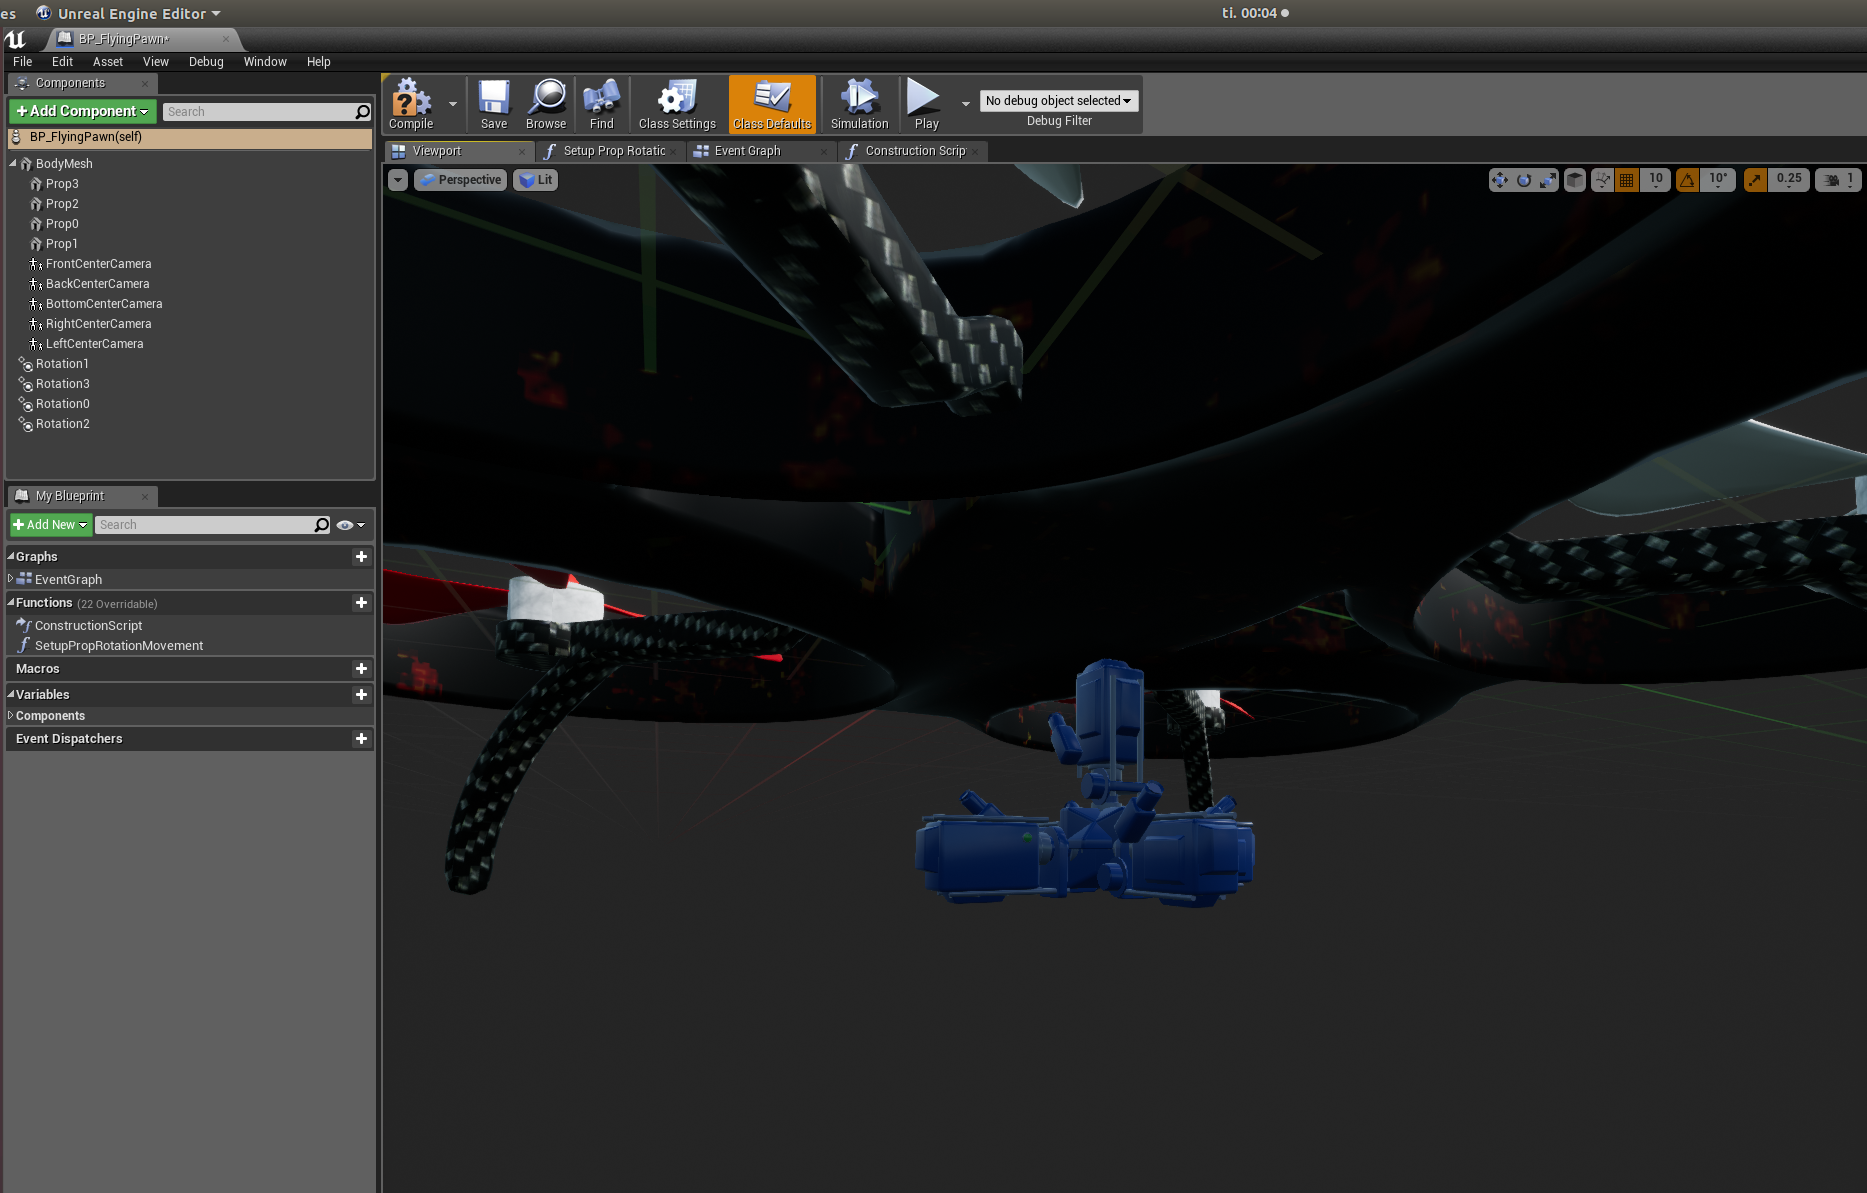
\includegraphics[height=4cm]{rapport/fig/Simulator/camera_setup.png}
        \caption{Fisheye camera setup}
        \label{fig:new_Blueprint_cameras}
    \end{subfigure}
    \begin{subfigure}{0.45\linewidth}
        \centering
        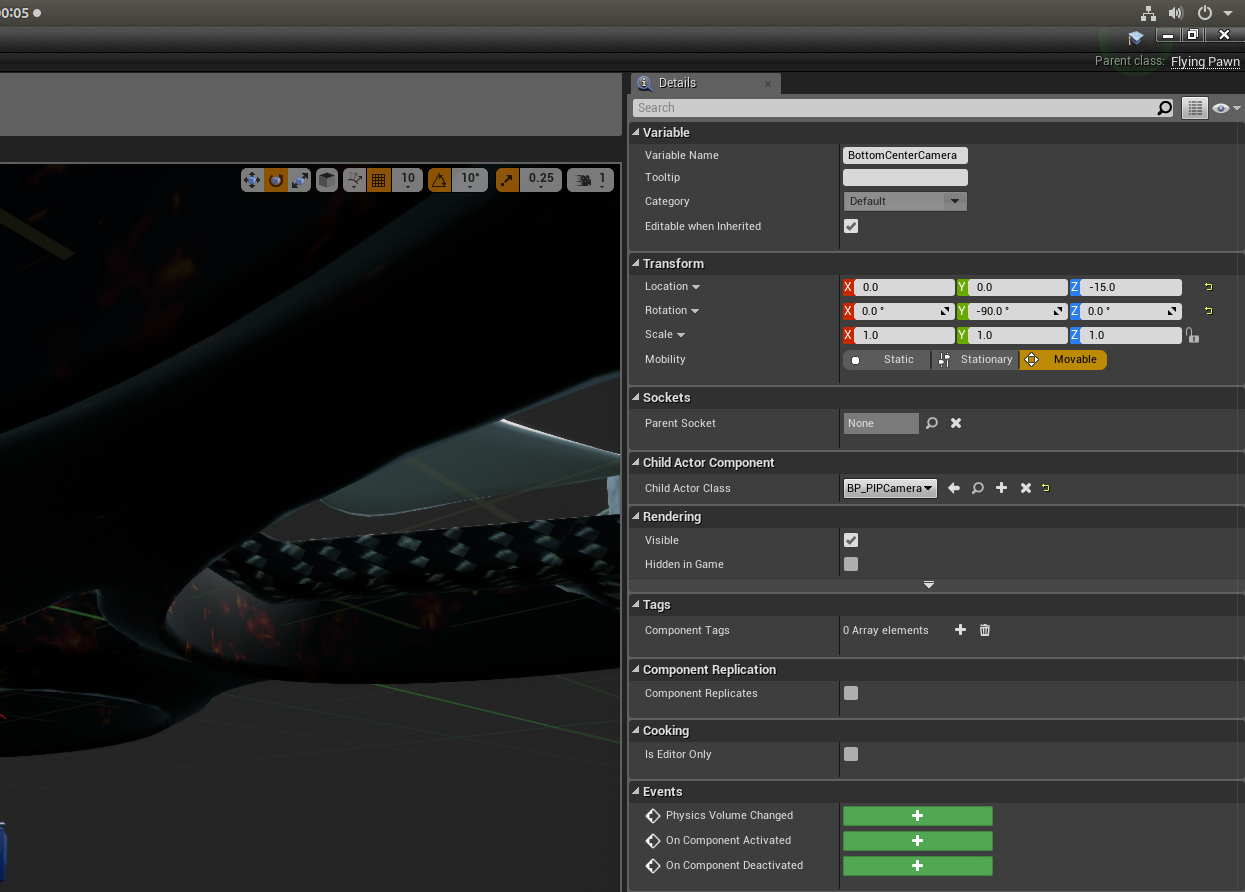
\includegraphics[height=4cm]{rapport/fig/Simulator/camera_setting.png}
        \caption{Downward camera settings}
        \label{fig:new_Blueprint_nodes}
    \end{subfigure}
    \caption{Multirotor Blueprint setup for the fisheye camera, consisting of 5 clustered perspective cameras.}
    \label{fig:new_Blueprint_multirotor}
\end{figure}

The following sections will present the modeling of the fisheye camera. The steps described are done on a pixel-wise level. As the same operation is done to every pixel in the source images, without any dependencies between them, this a highly parallelizable task, making it ideal for GPU accelereation.

\subsection{Combining pictures} \label{sec:combining_pictures}

The response form AirSim when requesting an image is an image response structure containing; camera name, position, orientation, time stamp, image dimensions, the image type and the image data. It also contains whether the image has been compressed to a PNG format. This field is however irrelevant as the fisheye camera will request raw RGBA8 pictures in order to do the mapping.

\begin{figure}[!htb]
    \centering
    \tdplotsetmaincoords{70}{160}
    \begin{tikzpicture}[tdplot_main_coords, scale = 1.4]
    
    \coordinate (O) at (0,0,0);
    \tdplotsetrotatedcoords{0}{-90}{90}
    
    \coordinate (IMBOTC) at (0,0,-2);
    \tdplotsetrotatedcoordsorigin{(IMBOTC)}
    \draw[tdplot_rotated_coords, thick, fill=black!8, opacity=1.0] (2,0,2) -- (2,0,-2) -- (-2,0,-2) -- (-2,0,2) -- cycle;
    
    \coordinate (IMLEFT) at (0,-2,0);
    \tdplotsetrotatedcoordsorigin{(IMLEFT)}
    \draw[tdplot_rotated_coords, thick, fill=black!8, opacity=1.0] (0,2,2) -- (0,-2,2) -- (0,-2,-2) -- (0,2,-2) -- cycle;
    
    
    \tdplotsetrotatedcoordsorigin{(O)}
    
    \draw[tdplot_rotated_coords, ->] (0,0,2) -- (0,0,3) node[below]{$Z$};
    
    \tdplotsetcoord{IMGC}{2}{-90}{0}
    \tdplotsetrotatedcoordsorigin{(IMGC)}
    \draw[thick, tdplot_rotated_coords, fill=black!4, opacity=0.8] (-2,-2,0) -- (-2,2,0) -- (2,2,0) -- (2,-2,0) -- cycle;
    
    \draw[tdplot_rotated_coords, dashed] (0,0,-1.5) -- (0,0,0);
    
    \draw[tdplot_rotated_coords, dashed, opacity=0.8] (0,0,-2) -- (0,-2,0);
    \draw[tdplot_rotated_coords, dashed, opacity=0.8] (0,0,-2) -- (2,0,0);
    \draw[tdplot_rotated_coords, dashed, opacity=0.8] (0,0,-2) -- (2,2,0);
    \draw[tdplot_rotated_coords, dashed, opacity=0.8] (0,0,-2) -- (2,-2,0);
    \draw[tdplot_rotated_coords, dashed, opacity=0.8] (0,0,-2) -- (-2,-2,0);
    
    \tdplotsetrotatedcoordsorigin{(O)}
    \tdplotsetrotatedcoords{90}{70}{0}
    \draw[tdplot_rotated_coords, thick, fill=black!5, opacity = 0.8] (0:2) arc (0:180:2);
    \tdplotsetrotatedcoords{0}{-90}{90}
    \draw[thick, tdplot_rotated_coords, fill=black!3] (0:2) arc (0:360:2);
    
    \tdplotsetrotatedcoords{0}{-90}{90}
    \draw[tdplot_rotated_coords, ->] (-0.5,0,0) -- (3,0,0) node[below]{$X$};
    \draw[tdplot_rotated_coords, ->] (0,-0.5,0) -- (0,2.5,0) node[right]{$Y$};
    \draw[tdplot_rotated_coords, dashed] (0,0,0) -- (0,0,0.6);
    
    \draw[tdplot_rotated_coords, dashed, opacity=0.8] (1.155,1.155,1.155) -- (2,2,2);
    \draw[tdplot_rotated_coords, dashed, opacity=0.8] (1.155,0,1.155) -- (2,0,2);
    \draw[tdplot_rotated_coords, dashed, opacity=0.8] (1.155,-1.155,1.155) -- (2,-2,2);
    
    \draw[tdplot_rotated_coords, dashed, opacity=0.8] (0,0,0) -- (0.5,0.5,0.5);
    \draw[tdplot_rotated_coords, dashed, opacity=0.8] (0,0,0) -- (0.5,0,0.5);
    \draw[tdplot_rotated_coords, dashed, opacity=0.8] (0,0,0) -- (0.5,-0.5,0.5);
    \draw[tdplot_rotated_coords, dashed, opacity=0.8] (0,0,0) -- (0,-0.6,0.6);
    \draw[tdplot_rotated_coords, dashed, opacity=0.8] (0,0,0) -- (-0.7,-0.7,0.7);
    
    
    \tdplotsetcoord{IMTOPC}{2}{0}{-90}
    \tdplotsetrotatedcoordsorigin{(IMTOPC)}
    \draw[tdplot_rotated_coords, thick, fill=black!2, opacity=0.7] (2,0,2) -- (2,0,-2) -- (-2,0,-2) -- (-2,0,2) -- cycle;
    
    \coordinate (IMRIGHT) at (0,2,0);
    \tdplotsetrotatedcoordsorigin{(IMRIGHT)}
    \draw[tdplot_rotated_coords, thick, fill=black!2, opacity=0.7] (0,2,2) -- (0,-2,2) -- (0,-2,-2) -- (0,2,-2) -- cycle;
    
    \end{tikzpicture}
    
    \caption{Projection from perspective camera to a unit sphere using 5 perspective cameras, given a FoV of $180^\circ$.}
    \label{fig:impl_Sphere_projection}
\end{figure}

Figure~\ref{fig:impl_Sphere_projection} shows the setup for the custom cube capture used by the fisheye camera, where each plane represent an image taken by a camera on the multirotor. To provide a correct projection, the angles $\phi$ and $\theta$, shown in Figure~\ref{fig:fisheye_spherical_projection} must be known. In order to convert the pixel positions to these angles, it is beneficial to change to image coordinates on a plane with $x^i,y^i \in [-1,1]$. Here $[x^i, y^i]^\top$ and $[u^i,v^i]^\top$ refer to the image and pixel coordinates on the image plane represented, with the origin in each camera's own coordinate frame. Table~\ref{tab:impl_quaternion_rotations} shows the respective superscripts used to describe each camera frame. Using Equation~\eqref{eq:pixel_transform}, with each camera having an aspect ratio $\rho = 1$, the transformation shown in Equation~\eqref{eq:impl_pixel_inverse_transform} is obtained.

\begin{equation}
    \mathbf{p}^i = \begin{bmatrix}
        x^i \\ y^i \\ 1
    \end{bmatrix} = \begin{bmatrix}
        \frac{W}{2} & 0 & \frac{W}{2} \\
        0 & \frac{H}{2} & \frac{H}{2} \\
        0 & 0 & 1
    \end{bmatrix}^{-1}\begin{bmatrix}
        u^i \\ v^i \\ 1
    \end{bmatrix} = \begin{bmatrix}
        \frac{2}{W} & 0 & -1 \\
        0 & \frac{2}{H} & -1 \\
        0 & 0 & 1
    \end{bmatrix}\begin{bmatrix}
        u^i \\ v^i \\ 1
    \end{bmatrix}
    \label{eq:impl_pixel_inverse_transform}
\end{equation}

A coordinate frame $\bullet^c$ is defined for the fisheye $360^\circ$ camera to be aligned with the coordinate frame of the downward pointing camera. Hence all points $\mathbf{p}^i = [x^i,y^i,z^i]^\top$, where $i$ refers to the superscript assigned to each camera frame, should be rotated to the camera frame. This rotation is shown in Equation~\eqref{eq:impl_rotation}. $\mathbf{R}^d_i$ represents the rotation from fra $i$ to $d$, where $\mathbf{q}_{d,i}$ in Equation~\eqref{eq:impl_rotation_q} represent the same rotation on quaternion form.

\begin{subequations}
    \begin{align}
        \mathbf{p}^c &= \!\begin{aligned}[t]
            \mathbf{p}^d = \begin{bmatrix} x^d \\ y^d \\ z^d \end{bmatrix} &= \mathbf{R}^d_i \mathbf{p}^i
        \end{aligned} \label{eq:impl_rotation_R} \\[0.75ex]
        \mathbf{q}^c &= \!\begin{aligned}[t]
            \mathbf{q}^d = \begin{bmatrix} 0 \\ \mathbf{p}^d \end{bmatrix} &= (\mathbf{q}_{d,i})\mathbf{q}^i(\mathbf{q}_{d,i})^\top
        \end{aligned} \label{eq:impl_rotation_q}
    \end{align}
    \label{eq:impl_rotation}
\end{subequations}

The quaternion rotation in Equation~\eqref{eq:impl_rotation_q} will be implemented in this project. Table~\ref{tab:impl_quaternion_rotations} lists each camera, their defined coordinate frame, as well as the rotation needed for the representative image coordinate vector. $\hat{\theta}$ and $\hat{\phi}$ represent the rotation angle around the local $x-$ and $y-$axis respectively.

\begin{table}[!htb]
    \centering
    \caption{Rotation needed to rotate image coordinate $p^i$ to $p^d$.}
    \label{tab:impl_quaternion_rotations}
    \begin{tabular}{|c|c|c|c|} \hline
        \multirow{2}{*}{Camera Direction} & \multirow{2}{*}{ $\mathbf{p}^i$} & \multirow{2}{*}{$\mathbf{R}^d_i = \mathbf{R}_{x,\hat{\theta}}(\hat{\theta})\mathbf{R}_{y,\hat{\phi}}(\hat{\phi})$} & \multirow{2}{*}{Quaternion $\mathbf{q}_{d,i}$} \\ &&& \\ \hline \hline
        \multirow{2}{*}{Down} & \multirow{2}{*}{$\mathbf{p}^d$} & \multirow{2}{*}{$\hat{\theta} = 0$, $\hat{\phi} = 0$} & \multirow{2}{*}{$[1,0,0,0]^\top$} \\ &&& \\ \hline
        \multirow{2}{*}{Front} & \multirow{2}{*}{$\mathbf{p}^f$} & \multirow{2}{*}{$\hat{\theta} = 90$, $\hat{\phi} = 0$} & \multirow{2}{*}{$\left[\frac{\sqrt{2}}{2},\frac{\sqrt{2}}{2},0,0\right]^\top$} \\ &&& \\ \hline
        \multirow{2}{*}{Right} & \multirow{2}{*}{$\mathbf{p}^r$} & \multirow{2}{*}{$\hat{\theta} = -90$, $\hat{\phi} = -90$} & \multirow{2}{*}{$[0.5,0.5,0.5,0.5]^\top$} \\ &&& \\ \hline
        \multirow{2}{*}{Back} & \multirow{2}{*}{$\mathbf{p}^b$} & \multirow{2}{*}{$\hat{\theta} = 180$, $\hat{\phi} = -90$} & \multirow{2}{*}{$\left[0,0,\frac{\sqrt{2}}{2},\frac{\sqrt{2}}{2}\right]^\top$} \\ &&& \\ \hline
        \multirow{2}{*}{Left} & \multirow{2}{*}{$\mathbf{p}^l$} & \multirow{2}{*}{$\hat{\theta} = 90$, $\hat{\phi} = -90$} & \multirow{2}{*}{$\left[0.5,0.5,-0.5,-0.5\right]^\top$} \\ &&& \\ \hline
    \end{tabular}
\end{table}

After rotating the image coordinate to the camera frame, the feature unit vector $[\theta, \phi]^\top$ can be calculated using Equation~\eqref{eq:theory_polar_coords}. This calculation is shown in Equation~\eqref{eq:impl_polar_transform}. The arctangent is implementing using the standard library \emph{atan2(y,x)} function. This provides extra functionality for calculating the quadrant of the angle. The result is therefore in the range $[-\pi,\pi]$, which is needed for correct picture placement.

\begin{subequations}
    \begin{equation}
        \theta = arctan\left(\frac{y^c}{x^c}\right)
        \label{eq:impl_polar_transform_theta}
    \end{equation}
    \begin{equation}
        \phi = arctan\left(\frac{\sqrt{(x^c)^2 + (y^c)^2}}{z^c}\right)
        \label{eq:impl_polar_transform_phi}
    \end{equation}
    \label{eq:impl_polar_transform}
\end{subequations}

\subsection{Lens implementation} \label{sec:lens_modeling}

The camera lens is implemented with the polynomial model presented in Table~11.1 in \cite{FisheyeCorke}. For now this is implemented as the fourth order polynomial in Equation~\eqref{eq:impl_lens_model}, where the paramers $k_1$-$k_4$ are tunable distortion parameters. $r(\phi)$ and $\theta$ refer to the polar coordinates of the fisheye image plane, defining the feature position in the fisheye image.

\begin{align}
    \begin{aligned}[t]
    r(\phi) &= k_1 \phi + k_2 \phi^2 + k_3 \phi^3 + k_4 \phi^4 \\[0.75ex]
    \theta &= \theta
    \end{aligned}
    \label{eq:impl_lens_model}
\end{align}

The polynomial model is quite flexible and easy to implement. While it does not support the more complex models, like the equisolid and stereographic models, these may be estimated through taylor expansion. The simple equiangular model used in the theory example in Equation~\eqref{eq:theory_equiangular_coords}, is found by setting $k_1 = f$, $k_2 = k_3 = k_4 = 0$.

In order to produce the final picture the polar coordinates have to be transformed back to pixel coordinates for the new image. Again using $W$ as the width and $H$ as the height in pixels, the transformation can be found using Equation~\eqref{eq:pixel_transform}, as well as the relationship between polar and Cartesian coordinates shown in Equation~\eqref{eq:theory_equiangular_coords}. The resulting transformation is shown in Equation~\eqref{eq:impl_pixel_transform_final}.

\begin{equation}
    \begin{bmatrix}
        u \\ v \\ 1
    \end{bmatrix} = \begin{bmatrix}
        \frac{W}{2x_{max}} & 0 & \frac{W}{2} \\
        0 & \frac{H}{2y_{max}} & \frac{H}{2} \\
        0 & 0 & 1
    \end{bmatrix}\begin{bmatrix}
        x \\ y \\ 1
    \end{bmatrix} =
    \begin{bmatrix}
        \frac{W}{2x_{max}} & 0 & \frac{W}{2} \\
        0 & \frac{H}{2y_{max}} & \frac{H}{2} \\
        0 & 0 & 1
    \end{bmatrix}\begin{bmatrix}
        r(\phi) cos(\theta) \\ r(\phi) sin(\theta) \\ 1
    \end{bmatrix}
    \label{eq:impl_pixel_transform_final}
\end{equation}

It can be seen from Equation~\eqref{eq:impl_lens_model} that the values for $y_{max}$ and $x_{max}$ can be calculated from Equation~\eqref{eq:impl_size_xy_max}. Since the maximum FoV is $270^\circ$.  $\phi_{max} = \frac{\theta}{2} = \left(\frac{3 \pi}{4}\right) rad$. This value is calculated with radians, as the powers of $270$ become quite large. Radians is also used in all the other trigonometric calculations for concistency and reducing human errors. 

\begin{equation}
    \begin{aligned}
        x_{max} = y_{max} &= ||k_1 \phi_{max} + k_2 \phi_{max}^2 + k_3 \phi_{max}^3 + k_4 \phi_{max}^4 ||_2 \\
        &= \left|\left| \left(\frac{3 \pi}{4}\right)k_1 + \left(\frac{3 \pi}{4}\right)^2 k_2 + \left(\frac{3 \pi}{4}\right)^3 k_3 + \left(\frac{3 \pi}{4}\right)^4 k_4 \right|\right|_2
    \end{aligned}
    \label{eq:impl_size_xy_max}
\end{equation}

One important thing to note about the scaling with $x_{max}$ or $y_{max}$ is that it removes some of the physical properties of the lens parameters. The fact that it scales the image plane to the pixel plane, removes potential mismatch between the sizes of the charge coupled device(CCD) and the projected image. Therefore, in order to simulate this effect and to calibrate the lens parameters correctly, the scaling should be disabled and substituted with the pixel dimensions on the actual CCD in the camera. This is shown in Equation~\eqref{eq:impl_pixel_transform_final_noscale}, where $w$ and $h$ refer to the physical dimensions of each pixel on the CCD, and $W$ and $H$ is referencing the width and height of the image in pixels.

\begin{equation}
    \begin{bmatrix}
        u \\ v \\ 1
    \end{bmatrix} = \begin{bmatrix}
        \frac{1}{w} & 0 & \frac{W}{2} \\
        0 & \frac{1}{h} & \frac{H}{2} \\
        0 & 0 & 1
    \end{bmatrix}\begin{bmatrix}
        x \\ y \\ 1
    \end{bmatrix} =
    \begin{bmatrix}
        \frac{1}{w} & 0 & \frac{W}{2} \\
        0 & \frac{1}{h} & \frac{H}{2} \\
        0 & 0 & 1
    \end{bmatrix}\begin{bmatrix}
        r(\phi) cos(\theta) \\ r(\phi) sin(\theta) \\ 1
    \end{bmatrix}
    \label{eq:impl_pixel_transform_final_noscale}
\end{equation}


% \subsection{Code structure}

% The fisheye module is made to be included as a library into other projects, along with it's header file. The module defines a FisheyeTransformer class and the Lens, SourceImage and TeansformRequest structures. SourceImage contains the one perspective 

% \begin{figure}
%     \centering
%     \begin{tikzpicture}[node distance = 4cm, transform shape, scale=1.0]
%         \tikzstyle{class} = [rectangle, minimum width=3cm, minimum height = 3cm, text centered, draw=black, fill=blue!10]
%         \tikzstyle{struct} = [rectangle, minimum width=3cm, minimum height = 3cm, text centered, draw=black, fill=green!10]
        
%         \node (FET) [class, align=center, rectangle split, rectangle split parts=2]{
%             \textbf{FisheyeTransformer}
%             \nodepart{second} \begin{flushleft}+\end{flushleft} test
%         };
        
%     \end{tikzpicture}
%     \caption{Caption}
%     \label{fig:my_label}
% \end{figure} Add this?

\subsection{ROS interface to AirSim and fisheye camera}\label{subsec:ROS_interface}

The ROS node implementation is split into two different parts. The first part handles the core loop of the program, sending AirSim ImageRequests and handling the fisheye transformations, while the other handles ROS publishing. To be able to do this the ROS package inherits the base RPC-Client API class defined for AirSim, along with including the ROS hrader, to create a link between the two. However, for the added functionality of publishing fisheye images, it also depends on the fisheye module, OpenCV and cv\_bridge\footnote{https://github.com/ros-perception/vision\_opencv}, where cv\_bridge handles the conversion between the OpenCV image object and the ROS image message.

\begin{figure}[!htb]
    \centering
    \begin{tikzpicture}[node distance=2cm, transform shape, scale=0.7]
        \tikzstyle{start} = [rectangle, rounded corners, minimum width = 2cm, minimum height = 1cm, text centered, draw=black, fill=red!10]
        \tikzstyle{if} = [diamond, minimum width = 2.5cm, minimum height = 1.5cm, text centered, draw=black, fill=blue!10]
        \tikzstyle{task} = [rectangle, rounded corners, minimum width = 3cm, minimum height = 1.5cm, text centered, draw=black, fill=blue!10]
        \tikzstyle{singlearrow} = [thick, ->, >=stealth]
        
        \node (START) [start]{Start};
        \node (CONN) [task, below of=START, align=center, yshift=0.45cm]{Connect to \\ mutlirotor};
        \node (PUBINIT) [task, below of=CONN, align=center]{Initialize \\ Publisher};
        
        \node (ROSOK) [if, below of=PUBINIT, yshift=-0.8cm]{ros::ok()?};
        \draw[] (ROSOK) node[xshift=1.7cm, yshift=0.3cm]{yes};
        \draw[] (ROSOK) node[xshift=0.5cm, yshift=-1.5cm]{no};
        \node (REQ) [task, align=center, right of=ROSOK, xshift=1.7cm]{Request \\ Images};
        \node (OPENCV) [task, align=center, right of=REQ, xshift=1.3cm]{Convert to \\ cv::Mat};
        \node (FISH) [task, align=center, right of=OPENCV, xshift=1.3cm]{Create \\ fisheye image};
        \node (CONV) [task, align=center, right of=FISH, xshift=1.75cm]{Convert to ROS \\ sensor\_msgs/Image};
        \node (PUB) [task, align=center, right of=CONV, xshift=1.75cm]{Publish to \\ /FisheyeImage};
        
        \node (DISC) [task, align=center, below of=ROSOK, yshift=-0.5cm]{Disconnect from \\ multirotor};
        \node (END) [start, below of=DISC, yshift=0.45cm]{End};
        
        \draw[singlearrow] (START) -- (CONN);
        \draw[singlearrow] (CONN) -- (PUBINIT);
        \draw[singlearrow] (PUBINIT) -- (ROSOK);
        \draw[singlearrow] (ROSOK) -- (REQ);
        \draw[singlearrow] (REQ) -- (OPENCV);
        \draw[singlearrow] (OPENCV) -- (FISH);
        \draw[singlearrow] (FISH) -- (CONV);
        \draw[singlearrow] (CONV) -- (PUB);
        \path[draw, -latex, singlearrow] (PUB) -- ++(0cm,1.7cm) -| (ROSOK);
        \draw[singlearrow] (ROSOK) -- (DISC);
        \draw[singlearrow] (DISC) -- (END);
        
    \end{tikzpicture}
    \caption{ROS publisher loop.}
    \label{fig:impl_ROS_pub_loop}
\end{figure}

Using the custom setup discussed in Section~\ref{subsec:Fisheye_impl_overview}, the requests for the perspective images are treated by referencing the cameras by name, as there is no way of polling AirSim to get the available cameras. The received vector of images is then converted to OpenCV images and wrapped into a custom FisheyeImageRequest made for this project. This structure holds the images, image size, and information about the camera pose, which is necessary to compute the final image.

The created ROS node runs an infinite loop, shown in Figure~\ref{fig:impl_ROS_pub_loop}. The loop is interruptable by crtl+c through the ros::ok() function. The loop consists of polling for images, conversion to fisheye image, and publishing the image on the FisheyImage ROS topic. In order to control the multirotor, the old client API needs to be included and used in the core loop of the client application. Both the ROS publisher and the old client API can run simultaneously.


\cleardoublepage

\chapter{Results and Discussion}

The simulator capture sets of five perspective images and converts them into one image, mimicking the effect of fisheye lenses cameras. Using the setup described in Section~\ref{sec:combining_pictures}, and an calibratable polynomial lens model, each images is mapped onto specific parts of the final fisheye image. In Figure~\ref{fig:res_show_fisheye} the complete image is shown, simulating a $270^\circ$ FoV camera, mounted beneath the multirotor during flight. The simulator is fully implemented for Linux, but will work on Windows with some modifications to the build system and client program. This includes removing the ROS publisher, as ROS is currently not available on Windows platforms. No part of the simulator has been tested on Mac OS. 

\begin{figure}[!htb]
    \centering
    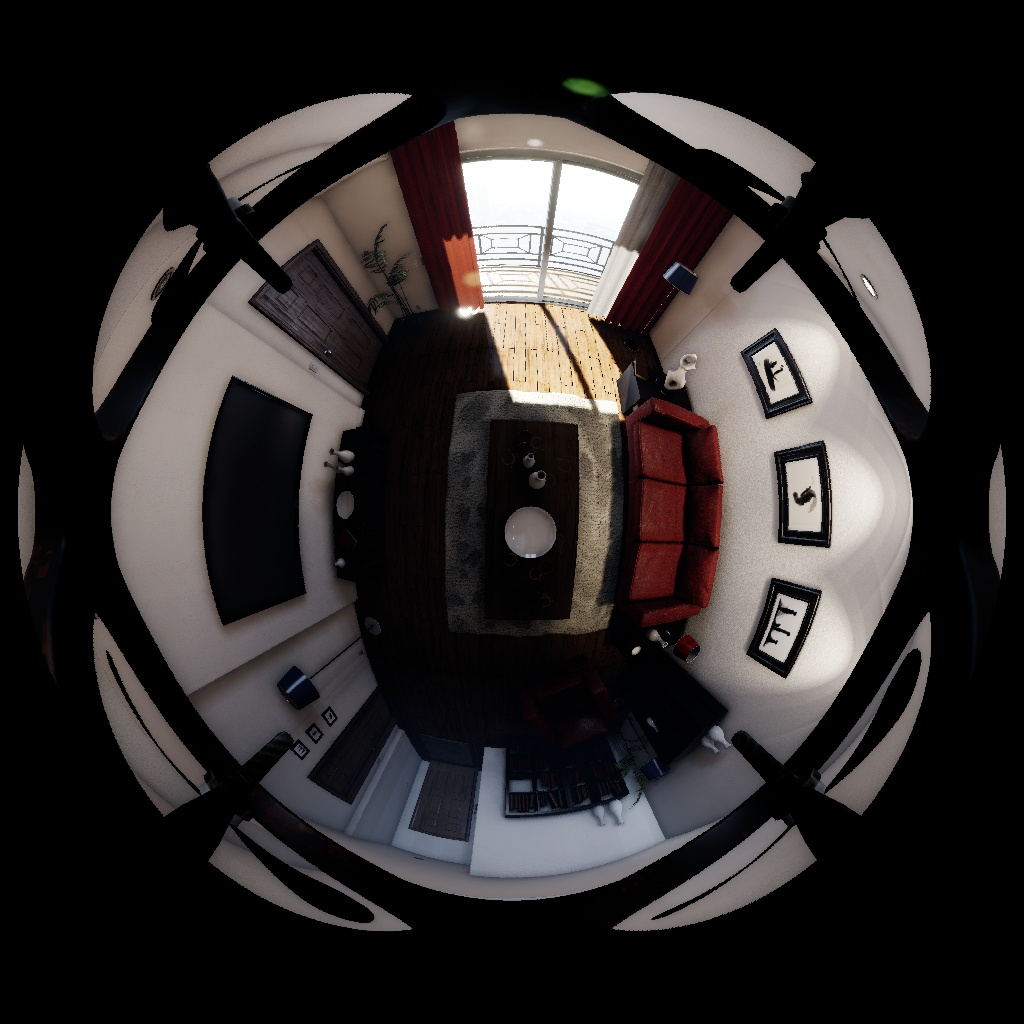
\includegraphics[width=0.7\textwidth]{rapport/fig/Results/1024to1024.jpeg}
    \caption{Simulated fisheye image taken in an indoor environment in Unreal Engine}
    \label{fig:res_show_fisheye}
\end{figure}

\section{Results}

The simulator is able to capture either single $90^\circ$ Fov pictures or full $270^\circ$ FoV pictures. This is because the simulator assumes the full five-camera setup, if it receives more than one image for transformation. The single pictures may be taken by any of the five cameras. This is donw by changing the image request sent to AirSim and setting the cameraposition as down, which tells the tranformer that the image does not need to be rotated.

The resolution settings for the perspective images can be set to a maximum of $4096\times4096$, and while there is no current limit to the resolution of the fisheye image, the height and width should should not exceed the double of the input image sizes. The FOV must equal $90^\circ$ for cube capture, but can be both increased and decreased for single captures, as long as the aspect ratio is preserved. 

\subsection{Fisheye captures and capture environment}

The images was taken in a indoor evironment provided by the Unreal Engine scene library. This is one of the freely available scenes in the Unreal Engine Library, and provides different types of lighting, some reflecting surfaces, as well as enough objects to be able to test the image quality. In Figure~\ref{fig:res_indoor_with_editor} the scene can be seen from editor view, while Figure~\ref{fig:res_original_pictures} shows five pictures taken from the multirotor inflight. All images shown in this comparison is taken with the default camera effect settings, which has a fast working auto exposure and no motion blur added. Picture noise is also tuned off.

\begin{figure}[!htb]
    \centering
    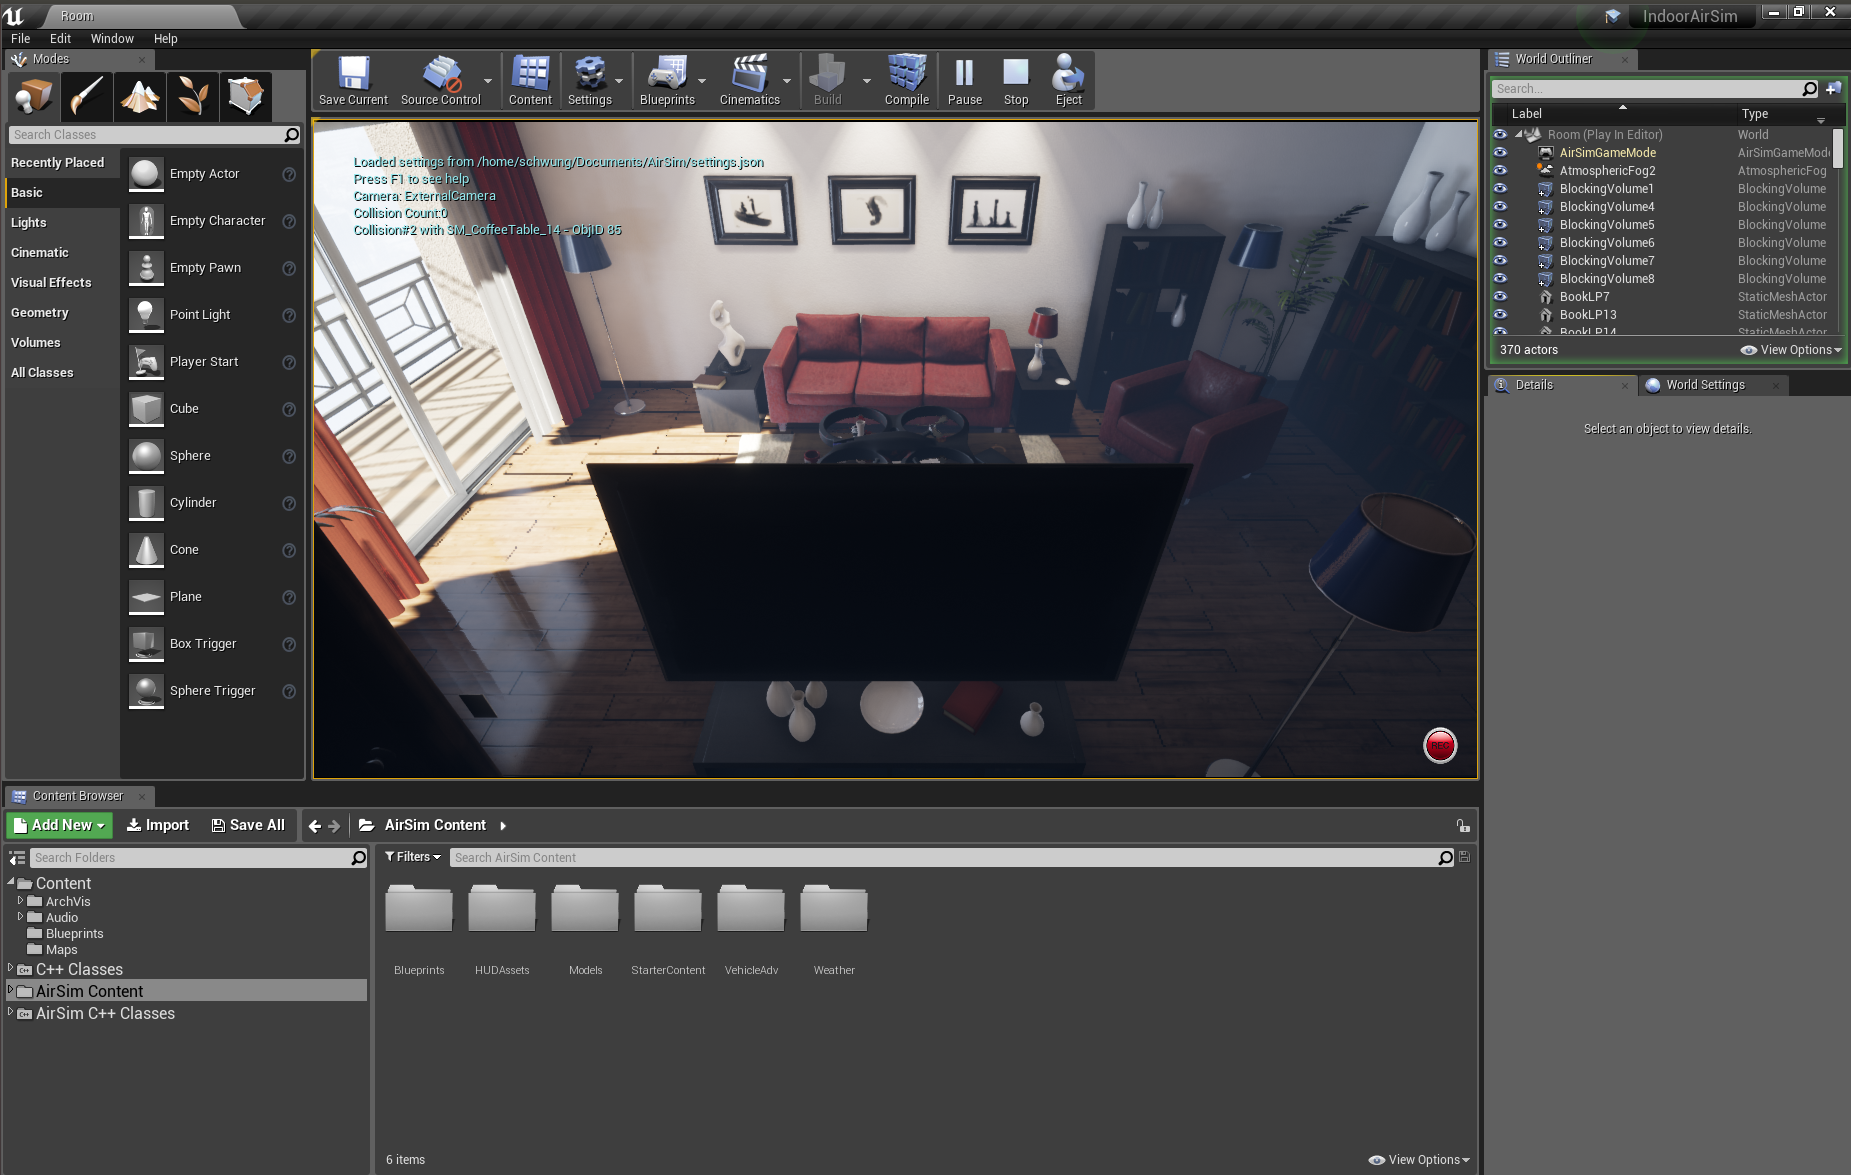
\includegraphics[width = 0.7\textwidth]{rapport/fig/Results/indoor_noconnect.png}
    \caption{Indoor test scene in the Unreal Engine editor}
    \label{fig:res_indoor_with_editor}
\end{figure}

The simulator will work in any environment created in Unreal Engine, by adding the project specific files along the AirSim files to the new scene. Figure \todo[inline]{add new environment} shows the same simulator in two other environments. The process of using pre-made scenes may be a bit tedious for Linux, since most scenes has been created for Windows. However, Unreal Engine provides tools for converting the projects to support Linux, and as of now all scenes have worked.

\begin{figure}[!htb]
    \centering
    \begin{subfigure}{0.32\textwidth}
    \centering
        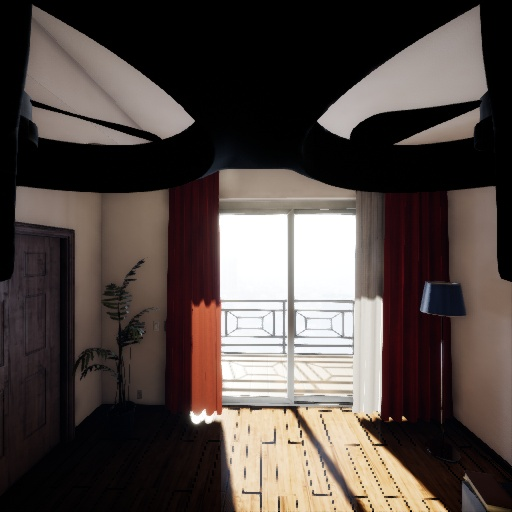
\includegraphics[height=5cm]{rapport/fig/Results/forward_center.jpeg}
        \caption{Front Camera}
        \label{fig:res_original_front}
    \end{subfigure}
    \begin{subfigure}{0.32\textwidth}
        \centering
        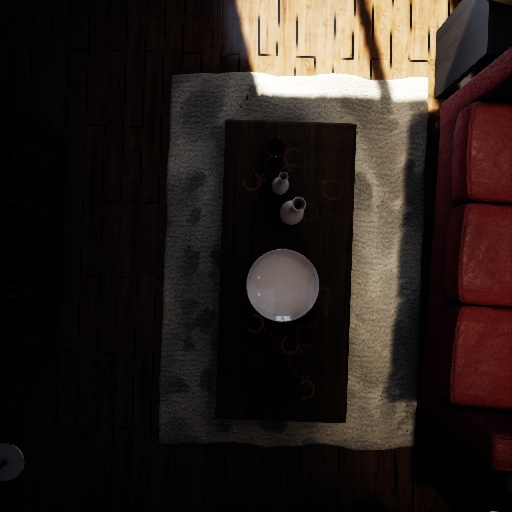
\includegraphics[height=5cm]{rapport/fig/Results/down_center.jpeg}
        \caption{Downward camera}
        \label{fig:res_original_down}
    \end{subfigure}    
    \begin{subfigure}{0.32\textwidth}
        \centering
        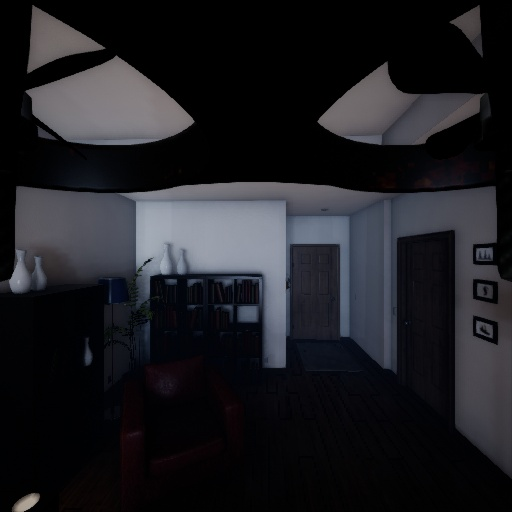
\includegraphics[height=5cm]{rapport/fig/Results/backward_center.jpeg}
        \caption{Back camera}
        \label{fig:res_original_back}
    \end{subfigure} \\[0.75ex]
    \begin{subfigure}{0.32\textwidth}
        \centering
        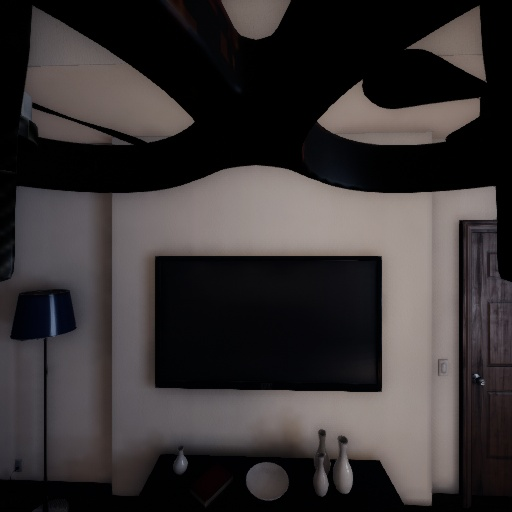
\includegraphics[height=5cm]{rapport/fig/Results/left_center.jpeg}
        \caption{Left Camera}
        \label{fig:res_original_left}
    \end{subfigure}
    \begin{subfigure}{0.32\textwidth}
        \centering
        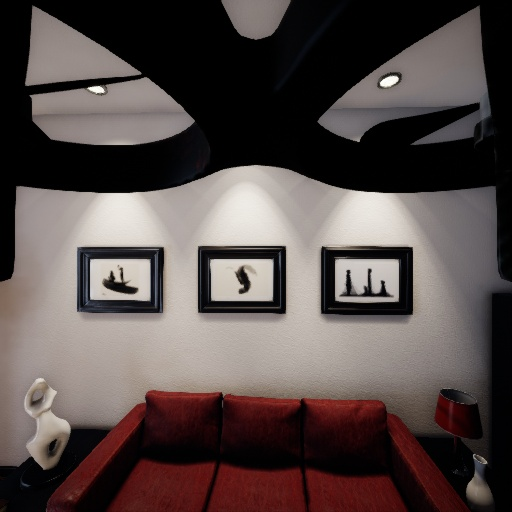
\includegraphics[height=5cm]{rapport/fig/Results/right_center.jpeg}
        \caption{Right Camera}
        \label{fig:res_original_right}
    \end{subfigure}
    \centering
    \caption{Comparison of image quality in different resolutions}
    \label{fig:res_original_pictures}
\end{figure}

In Figure~\ref{fig:res_quality_comparison} we see three images taken with different resolution, and using the lens parameters; $k_1 = 1.0$, $k_2=k_3=k_4=0$, creating an equiangular projection. The resolution in the compared pictures matches that of the perspective image resolution. This means that the $512\times512$ pixel image is combined from five $512\times512$ pixel images and so on. One can see that the image in Figure~\ref{fig:res_comp_256_to_256} is substantially lower than that of the image in Figure~\ref{fig:res_comp_1024_1024}. Almost all details on the door and railing are lost, and the reflection seen in the plate at the table is almost none existent. Comparing Figure~\ref{fig:res_comp_512_512} and Figure~\ref{fig:res_comp_1024_1024}, the differences are quite minimal.

\begin{figure}[!htb]
    \centering
    \begin{subfigure}{0.32\textwidth}
    \centering
        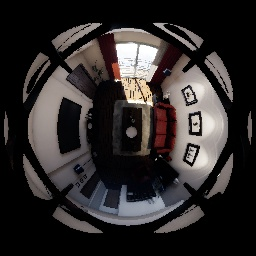
\includegraphics[height=5cm]{rapport/fig/Results/256to256.jpeg}
        \caption{$256 \times 256$ pixels}
        \label{fig:res_comp_256_to_256}
    \end{subfigure}
    \begin{subfigure}{0.32\textwidth}
        \centering
        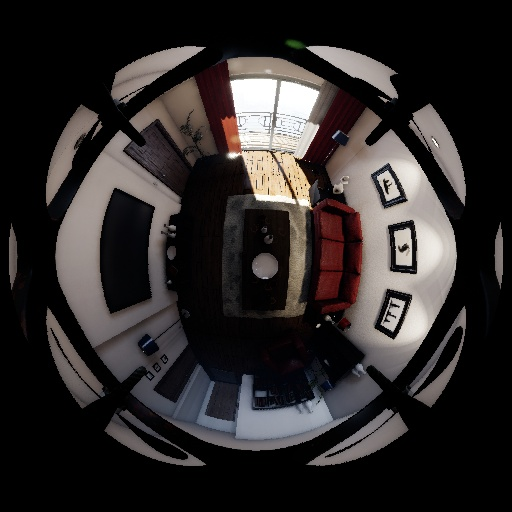
\includegraphics[height=5cm]{rapport/fig/Results/512to512.jpeg}
        \caption{$512 \times 512$ pixels}
        \label{fig:res_comp_512_512}
    \end{subfigure}    
    \begin{subfigure}{0.32\textwidth}
        \centering
        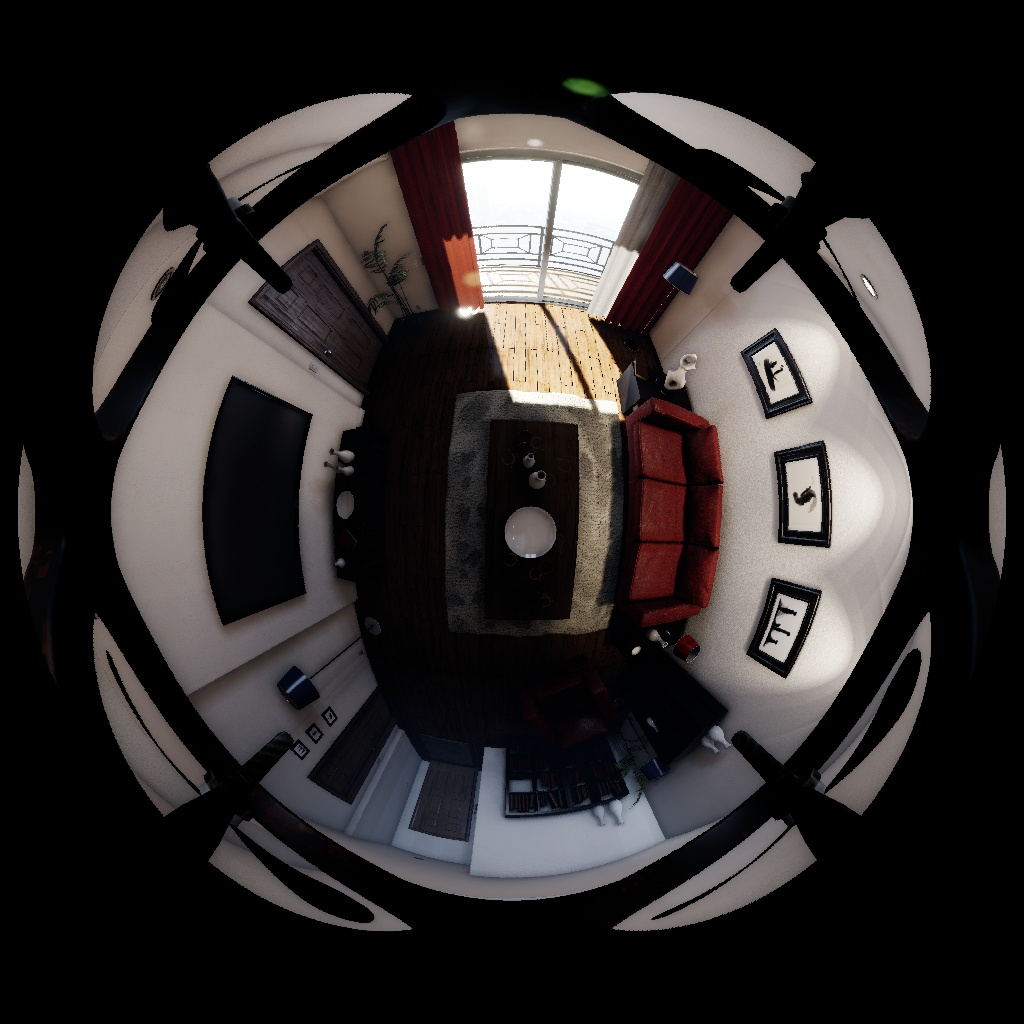
\includegraphics[height=5cm]{rapport/fig/Results/1024to1024.jpeg}
        \caption{$1024 \times 1024$ pixels}
        \label{fig:res_comp_1024_1024}
    \end{subfigure}
    \centering
    \caption{Comparison of image quality in different resolutions}
    \label{fig:res_quality_comparison}
\end{figure}

The images in Figure~\ref{fig:res_comp_equal} are taken with the same perspective image resolution of $512 \times 512$, but with two different destination resolutions. The most important difference here is the distortion lines seen in Figure~\ref{fig:res_comp_equal_512_1024}, caused by the stretching of the source image. However, it can also be seen that the detail level in the central parts have been increased.

\begin{figure}[!htb]
    \centering
    \begin{subfigure}{0.45\textwidth}
        \centering
        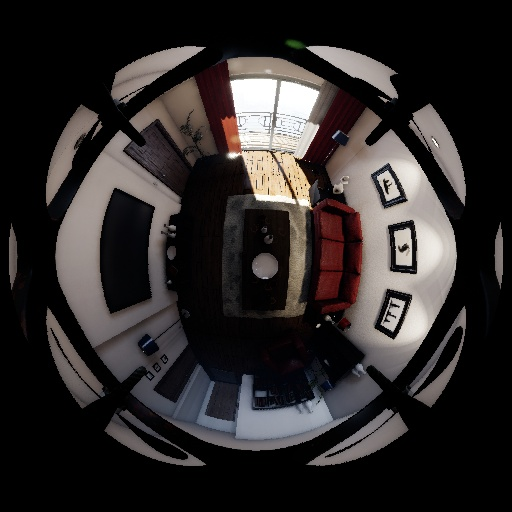
\includegraphics[height=7cm]{rapport/fig/Results/512to512.jpeg}
        \caption{$512 \times 512$ pixels}
        \label{fig:res_comp_equal_512_512}
    \end{subfigure}
    \begin{subfigure}{0.45\textwidth}
        \centering
        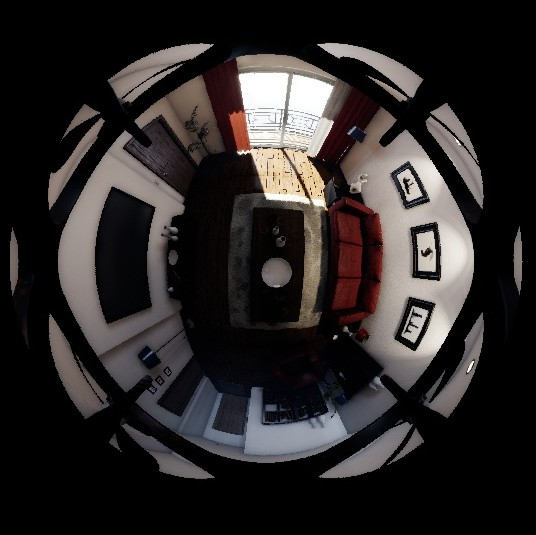
\includegraphics[height=7cm]{rapport/fig/Results/512to1024.jpeg}
        \caption{$1024 \times 1024$ pixels}
        \label{fig:res_comp_equal_512_1024}
    \end{subfigure}
    \caption{Comparison of transformed images with equal source resolution of $512 \times 512$}
    \label{fig:res_comp_equal}
\end{figure}

\subsection{Performance}

While the performance never was a part of the equation when implementing it, it is an important factor in a control application. All tests have been performed on the office PC in at NTNU. This PC does not have a dedicated graphics card, and Unreal Engine lagged considerably during tests. How much this affected the tests is unknown. however they should show qualitative data to shed some light upon areas to imporve the simulator.

Table~\ref{tab:res_timing_single} and \ref{tab:res_timing_cube_capture} show the timings in seconds for different resolutions and capture types. Note that while this is not even close to real time, all calculations done by the simulator are done sequentially for each pixel in the picture, meaning that no parallellization has been done. This can clearly be seen by comparing the calculation times, where the computation time follows the increase in resolution linearly. The fetch times are also higher for higher resolution picture, which are to be expected. Around $512\times 512$ it became quite noticable. 

\begin{table}[!htb]
    \centering
    \begin{tabular}{|c|c|c|c|} \hline
        \textbf{Input resolution} & \textbf{output resolution} & \textbf{Timing type} & \textbf{Time elapsed} \\ \hline \hline
        \multirow{2}{*}{$256 \times 256$} & \multirow{2}{*}{$512 \times 512$} & Fetch & 0.1 - 0.2 s \\ \cline{3-4}
         & & Transform & 0.4 s \\ \hline
        \multirow{2}{*}{$512 \times 512$} & \multirow{2}{*}{$512 \times 512$} & Fetch & 0.1 - 0.2 s\\ \cline{3-4}
         & & Transform & 1.5 s \\ \cline{2-4}
        \multirow{2}{*}{$1024 \times 1024$} & \multirow{2}{*}{$1024 \times 1024$} & Fetch &  0.3 - 0.5 s \\ \cline{3-4}
         & & Transform & 6.0 s \\ \hline
        \multirow{2}{*}{$2048 \time 2048$} & \multirow{2}{*}{$2048 \times 2048$} & Fetch & 0.6 - 0.7 s\\ \cline{3-4}
         & & Transform & 24.1 s\\ \hline
    \end{tabular}
    \caption{Timing for single capture transformation to fisheye image}
    \label{tab:res_timing_single}
\end{table}

\begin{table}[!htb]
    \centering
    \begin{tabular}{|c|c|c|c|} \hline
        \textbf{Input resolution} & \textbf{output resolution} & \textbf{Timing type} & \textbf{Time elapsed} \\ \hline \hline
        \multirow{2}{*}{$256 \times 256$} & \multirow{2}{*}{$256 \times 256$} & Fetch & 0.3 - 0.4 s\\ \cline{3-4}
         & & Transform & 2.0 s\\ \hline
        \multirow{4}{*}{$512 \times 512$} & \multirow{2}{*}{$512 \times 512$} & Fetch & 0.4 - 0.5 s \\ \cline{3-4}
         & & Transform & 7.9 s\\ \cline{2-4}
         & \multirow{2}{*}{$1024 \times 1024$} & Fetch & 0.4 - 0.5 s\\ \cline{3-4}
         & & Transform & 7.9 s\\ \hline
        \multirow{2}{*}{$1024 \time 1024$} & \multirow{2}{*}{$1024 \times 1024$} & Fetch & 0.7 s\\ \cline{3-4}
         & & Transform & 30.9 s\\ \hline
    \end{tabular}
    \caption{Timing for cube capture transformation to fisheye image}
    \label{tab:res_timing_cube_capture}
\end{table}


\section{Discussion}



\subsection{Image Quality}

\subsection{Performance and optimization}

\subsection{Task}

This project has not been a typical cybernetics project, and in many ways it shares more similarities with a computer science project. While the goal of was to extend the project to incorporate calibrating the fisheye camera to an actual camera, and possiby test computer vision algorithms on the platform, there hasn't been time. This is mainly because of lack of experience in critical areas. 

The project has had to handle very large code bases. Both the codebase of Unreal Engine and AirSim is quite extensive, as they both provide lots of functionality and features. While both platforms have a large user base, few of these discuss problems around the source code and the communication patterns within. Information regarding this is mostly limited to Github issues, and a few forum posts. While these problems became less relevant when making the client side application, it was a huge part of the development described in Section~\ref{sec:Early_dev}. 

Since the fisheye model was to be included into the AirSim interface, a deep understanding of the AirSim package was needed. Both in terms of internal dependencies, class and type definitions, coding style and communication patterns. The fact that it also had to incorporate new funtionality fom Unreal Engine meant that knowledge of C++ scripting towards Unreal Engine was needed. As the platform has an enormous amount of tools and funtionality available, there are also a lot of abstractions, to make the interface possible to use and develop for. However, the lack of previous experiece with game engines or Unreal Engine in particular, made this process quite time consuming. While reading through guides and watching tutorials

\subsection{Platform}

% This decision was made in order to separate the implementation into its own module, and thereby reducing the impact of changes to AirSim. As AirSim is still developed heavilly upon, it was seen as a way to reduce the amount trouble induced by changes to the core code of the plugin. This would also allow me to more often integrate the bug fixes and new implementations they made, without ruining my ownw work. The downside of this decision is that it removes possibility to use any features in Unreal Engine which is not implemented in the AirSim API. 


% \subsection{Project setup and programming environment}

% In this project I have forked both the EpicGames/Unreal Engine and the Microsoft/AirSim repository to my Github account, and made my own pivate repository for the project. This enable me to do specific changes to the source code of these projects, without the need to make pull requests to their original repositories. While AirSim is openly available, the source code of Unreal Engine is only available after being registered as a developer through their website. One requirement for getting the source code is that it is not distributed outside of this licencing. For this reason neither the fork of Unreal Engine, nor my own project repository are publicly available.

% Since one of the main goals of this project is the interfacing to ROS, the main OS for development will be Linux, specifically Ubuntu 18.04. However, since Unreal Engine is deeply integrated with Visual Studios, I will use Visual Studios on Windows as the main debugging platform, for everything except ROS. To build on Linux, I will use CMake, as they have done with AirSim. Both Unreal Engine and AirSim is built with the clang compiler, using libc++ as the standard library. However, the default ROS install uses libstdc++ as their standard library. This caused linking problems when combining ROS and AirSim. I therefore had to make some changes to the build and CMake scripts of AirSim in order to build with the GNU compiler g++, using libstdc++ as the standard library.

% \todo[inline]{Do I need to describe why this change is important?}

\cleardoublepage
%===================================== CHAP 5 =================================

\chapter{Conclusion and future work}
\section{Conclusion}
As stated in Section~\ref{chap:introduction}, there are no existing simulators for capturing wide-angle images with a FoV larger than 180 degrees today. As the results show in Section~\ref{sec:Results} proves, this task has been achieved. Utilizing the power of the Unreal Engine, it is also able to capture natural looking images with added effects, caused by light in the real world, such as lens flares, varying light conditions and effects of shadows and reflection. Especially the effects seen in Figure~\ref{fig:res_comp_single}, where the camera is exposed to sharp direct light are interesting topics that are simulatable on this platform.

While it may have been easier to implement the simulator in a simulator like Gazebo, the added amount of possibilities of CV applications using Unreal Engine is enough to justify the increased development time by itself, especially as powerful graphics cards become more and more commercially available. Having the available GPU accelerated function library of Unreal Engine may also be beneficial for further advancements to the platform.

As the transformations can be pre-calculated before the simulation starts, there is only one bottleneck left to remove. The fact that the fetching of images can take over half a second is not applicable for real-time simulation. One theory is that the RPC server/client architecture gets overloaded by the amount of picture data that is sent and therefore creates a bottleneck. If this proves to be true, then the fisheye model needs to be rewritten into the Unreal Engine game loop of AirSim. This might prove beneficial to do anyway, because of the aforementioned function library of Unreal Engine.

The original plan of implementing the simulator as a part of AirSim, rather than a client application, was not achieved due to the author's inexperience with C++, Unreal Engine and AirSim. However choosing to make the fisheye transformer as a client-side module enables it to be exported easily to other projects that need this kind picture mapping, as the module itself does not depend on either AirSim or Unreal Engine. This decision did unfortunately also limit the simulator to not be able to use the functionality of Unreal Engine directly, meaning that all post-processing had to be done before the transformation. For most light based effects this is of little consequence. However, it turned out that the added noise effects become warped and unnatural looking in the final picture. Another problem that remains to be solved is the motion blur effect, and why it does not work as intended. Further research into the post-processing of Unreal Engine is therefore needed in order to achieve this important feature. 

All in all the results show that the simulator is able to transform perspective images into a realistic looking fisheye image, with a 270-degree FoV, opening up for testing of CV algorithms for wide angle imaging in realistic light conditions. While the simulator still is in an early development state, the work presented should provide a suitable framework for further advancements.

\section{Future work}

Even though the possibilities for extensions to this module are numerous. Some problems have to be fixed first. These include:
\begin{itemize}
    \item Finalizing the mapping function for linear time picture transformation
    \item Removing the bottleneck in the picture fetching stage
    \item Finding the problem of motion blur
    \item Adding a noise model that is usable with the fisheye pictures
\end{itemize}

Dependent on the results of the aforementioned points, there may also be a need to implement the module without the dependency on RPC.

Assuming these problems can be solved, it would be very interesting to test captured images in the simulator against images captured with fisheye-cameras in the real world and to calibrate an actual camera in the simulator. This could also be extended to implementing SLAM and VO-algorithms on this platform, while comparing the results to other simulators and real tests.

Looking into Graphics programming for graphics accelerated multi-thread support would be a nice feature, as this may reduce the startup time of the simulator significantly. OpenCL and CUDA are two examples of programming libraries used to do this. While OpenCL supports many different GPU architectures, CUDA only supports NVidia GPUs. In this project, almost all matrix calculations and quaternion rotations are computed through Eigen, while the image specific matrices are handled by OpenCV. Both of these have added support for CUDA and OpenGL. This means that only the program loop itself needs to be parallelized.

While most fisheye lenses are made to create equiangular projections, lenses are not ideal. This means that other distortion effects that are not radial should also be implemented in the simulator. One possibility is to add the unified model proposed by \cite{FisheyeKalibration}. This adds additional distortion possibilities as well as also supporting catadioptric lenses.

Both catadioptric and panomorph lenses would be a nice addition to the simulator, which could be added without too much work. The catadioptric camera needs some extra logic for its blind spot, while the panomorph camera most likely could be added by estimating it in the polynomial model, as well as adding stretch parameters to the lens.

The Ros publisher is currently quite basic. While it can publish images to the ROS network, that is also everything it is able to do. Implementing multirotor controls into this framework would be preferable. This way one could control the whole simulation from ROS. Adding the supported sensors from AirSim into this publisher node would also add a lot of control application possibilities in the future.

Adding a more modular camera module would be really beneficial. As of now, the camera setup needs to be made each time a new vehicle is implemented, where the cameras are tied to that specific vehicle. Using Blueprints to make a standardized camera setup for fisheye capture would be nice, as it would also create a modular interface for others that may want to improve the platform.

As of now, only the multirotor mode of AirSim is supported for fisheye image capture. Adding this functionality to the other vehicles should not be too difficult, now that the platform exists for one vehicle. Of course, the addition of the camera setup blueprint mentioned earlier would also help to speed up this process.

The number of vehicles available for AirSim is quite limited. Adding new vehicles, for example a boat and a plane would widen the applications of the simulator. This is a large task, as this requires both 3D-modeling, custom scripting towards Unreal Engine, and the creation of new physics to tie into AirSim's already existing framework.

Unreal Engine recently partnered with NVidia during the release of their new graphics hardware to support real-time ray tracing into their platform. Based on their launch event presentation \cite{NvidiaConference}, this will be realized by the integration of so-called ray tracing cores, a specialized ray tracing acceleration algorithm and deep learning. Where the deep learning part is specifically made to upscale sparsely ray-traced scenes. Following this work might be interesting for the future of the platform, as well as the realism of the scenes. This will however not be available for some time.



\cleardoublepage

% \subsection{Task}

% This project has not been a typical cybernetics project, and in many ways it shares more similarities with a computer science project. While the goal of was to extend the project to incorporate calibrating the fisheye camera to an actual camera, and possiby test computer vision algorithms on the platform, there hasn't been time. This is mainly because of lack of experience in critical areas. 

% The project has had to handle very large code bases. Both the codebase of Unreal Engine and AirSim is quite extensive, as they both provide lots of functionality and features. While both platforms have a large user base, few of these discuss problems around the source code and the communication patterns within. Information regarding this is mostly limited to Github issues, and a few forum posts. While these problems became less relevant when making the client side application, it was a huge part of the development described in Section~\ref{sec:Early_dev}. 

% Since the fisheye model was to be included into the AirSim interface, a deep understanding of the AirSim package was needed. Both in terms of internal dependencies, class and type definitions, coding style and communication patterns. The fact that it also had to incorporate new funtionality fom Unreal Engine meant that knowledge of C++ scripting towards Unreal Engine was needed. As the platform has an enormous amount of tools and funtionality available, there are also a lot of abstractions, to make the interface possible to use and develop for. However, the lack of previous experiece with game engines or Unreal Engine in particular, made this process quite time consuming. While reading through guides and watching tutorials



% \subsection{Project setup and programming environment}

% In this project I have forked both the EpicGames/Unreal Engine and the Microsoft/AirSim repository to my Github account, and made my own pivate repository for the project. This enable me to do specific changes to the source code of these projects, without the need to make pull requests to their original repositories. While AirSim is openly available, the source code of Unreal Engine is only available after being registered as a developer through their website. One requirement for getting the source code is that it is not distributed outside of this licencing. For this reason neither the fork of Unreal Engine, nor my own project repository are publicly available.

% Since one of the main goals of this project is the interfacing to ROS, the main OS for development will be Linux, specifically Ubuntu 18.04. However, since Unreal Engine is deeply integrated with Visual Studios, I will use Visual Studios on Windows as the main debugging platform, for everything except ROS. To build on Linux, I will use CMake, as they have done with AirSim. Both Unreal Engine and AirSim is built with the clang compiler, using libc++ as the standard library. However, the default ROS install uses libstdc++ as their standard library. This caused linking problems when combining ROS and AirSim. I therefore had to make some changes to the build and CMake scripts of AirSim in order to build with the GNU compiler g++, using libstdc++ as the standard library.

% \todo[inline]{Do I need to describe why this change is important?}

%% PART 4
\pagestyle{fancy}
\fancyhf{}
\renewcommand{\chaptermark}[1]{\markboth{\chaptername\ \thechapter.\ #1}{}}
\renewcommand{\sectionmark}[1]{\markright{\thesection\ #1}}
\renewcommand{\headrulewidth}{0.1ex}
\renewcommand{\footrulewidth}{0.1ex}
\fancyfoot[LE,RO]{\thepage}
\fancypagestyle{plain}{\fancyhf{}\fancyfoot[LE,RO]{\thepage}\renewcommand{\headrulewidth}{0ex}}

\addcontentsline{toc}{chapter}{Bibliography}

\bibliographystyle{elsarticle-harv}
\bibliography{mylib}

\cleardoublepage	%% Edit your references in "mylib.bib"
%\section*{\begin{center}{\Huge Appendix}\end{center}}
\addcontentsline{toc}{chapter}{Appendix}
$\\[0.5cm]$

\noindent Write your appendix here...

\end{document}